%%%%%%%%%%%%%%%%%%%%%%%%%%%%%%%%%%%%%%%%%%%%%%%%%%%%%%%%%%%%%%%%
%%%%%%%%%%%%%%%%%%%%%%%%%%%%%%%%%%%%%%%%%%%%%%%%%%%%%%%%%%%%%%%%
%%%%%%%%%%%%%%%%%%%%%%%%%%%%%%%%%%%%%%%%%%%%%%%%%%%%%%%%%%%%%%%%
%%%%%%%%%%%%%%%%%%%%%%%%%%%%%%%%%%%%%%%%%%%%%%%%%%%%%%%%%%%%%%%%
\chapter[Systèmes linéaires, continus\ldots]{Systèmes linéaires continus et invariants\label{chap-slci}}
%%%%%%%%%%%%%%%%%%%%%%%%%%%%%%%%%%%%%%%%%%%%%%%%%%%%%%%%%%%%%%%%
%%%%%%%%%%%%%%%%%%%%%%%%%%%%%%%%%%%%%%%%%%%%%%%%%%%%%%%%%%%%%%%%
%%%%%%%%%%%%%%%%%%%%%%%%%%%%%%%%%%%%%%%%%%%%%%%%%%%%%%%%%%%%%%%%
%%%%%%%%%%%%%%%%%%%%%%%%%%%%%%%%%%%%%%%%%%%%%%%%%%%%%%%%%%%%%%%%
\adjustmtc
\minitoc
\newpage
%%%%%%%%%%%%%%%%%%%%%%%%%%%%%%%%%%%%%%%%%%%%%%%%%%%%%%%%%%%%%%%%
%%%%%%%%%%%%%%%%%%%%%%%%%%%%%%%%%%%%%%%%%%%%%%%%%%%%%%%%%%%%%%%%
%%%%%%%%%%%%%%%%%%%%%%%%%%%%%%%%%%%%%%%%%%%%%%%%%%%%%%%%%%%%%%%%
\section{Introduction}
%%%%%%%%%%%%%%%%%%%%%%%%%%%%%%%%%%%%%%%%%%%%%%%%%%%%%%%%%%%%%%%%
%%%%%%%%%%%%%%%%%%%%%%%%%%%%%%%%%%%%%%%%%%%%%%%%%%%%%%%%%%%%%%%%
%%%%%%%%%%%%%%%%%%%%%%%%%%%%%%%%%%%%%%%%%%%%%%%%%%%%%%%%%%%%%%%%
Dans ce chapitre, nous présentons les outils mathématiques 
et notions fondamentales pour la \textbf{modélisation} de l'automatique.

Dans un premier temps, nous donnerons une définition de chacuns 
des termes qui compose la notion centrale de \gls{slci} ainsi que quelques
exemples classiques de système électronique ou mécanique.
Nous aborderons les différents signaux usuels rencontrés
en automatique\footnote{et en traitement du signal de façon générale.}.
Ce chapitre nous permettra d'introduire la transformée de Laplace qui 
est l'outils mathématique indispensable de l'automaticien.
Celle-ci nous conduiera naturellement à la définition 
de la \textbf{fonction de transfert} qui caractérisera de façon univoque 
les systèmes dynamiques linéaires.

\begin{figure}[!h]
\begin{center}
    \tikzsetnextfilename{systeme-chap0-ext}
    \tikzsetnextfilename{systeme-chap0-ext}
\begin{tikzpicture}
\tikzset{sys/.style={draw,
					 minimum width=5cm,
					 minimum height=3cm,
					 rounded corners=15pt,
					 inner sep=0.5pt,
					 text width=4cm,
					 align=center}
}
\node[sys,ultra thick] (S) at (0,0) {\LARGE\scshape Système};
\node[above of=S,yshift=4em]  {\large Perturbations};
\node[below of=S,yshift=-4em] {\large Mesures};
\node[left of=S,xshift=-8em,yshift=2.5em]  (e1) {\large Entrée 1};
\node[left of=S,xshift=-8em,yshift=1em]    (e2) {\large Entrée 2};
\node[left of=S,xshift=-8em,yshift=-0.5em] (ed) {\large \rotatebox{90}{\ldots}};
\node[left of=S,xshift=-8em,yshift=-2em]   (en) {\large Entrée n};
\draw[-{Latex[length=2.5mm]}] (e1) -- (e1-|S.west);
\draw[-latex] (e2) -- (e2-|S.west);
\draw[-latex] (en) -- (en-|S.west);
\node[right of=S,xshift=8em,yshift=2.5em]  (s1) {\large Sortie 1};
\node[right of=S,xshift=8em,yshift=1em]    (s2) {\large Sortie 2};
\node[right of=S,xshift=8em,yshift=-0.5em] (sd) {\large \rotatebox{90}{\ldots}};
\node[right of=S,xshift=8em,yshift=-2em]   (sn) {\large Sortie n};
\draw[latex-] (s1) -- (s1-|S.east);
\draw[latex-] (s2) -- (s2-|S.east);
\draw[latex-] (sn) -- (sn-|S.east);
\node[above of=S,yshift=3.5em,xshift=-4em] (p1) {};
\node[above of=S,yshift=3.5em,xshift=-2em] (p2) {};
\node[above of=S,yshift=3.5em,xshift=0em]  (p3) {};
\node[above of=S,yshift=3.5em,xshift=2em]  (p4) {};
\node[above of=S,yshift=3.5em,xshift=4em]  (p5) {};
\draw[-latex] (p1) -- (p1|-S.north);
\draw[-latex] (p2) -- (p2|-S.north);
\draw[-latex] (p3) -- (p3|-S.north);
\draw[-latex] (p4) -- (p4|-S.north);
\draw[-latex] (p5) -- (p5|-S.north);
\node[below of=S,yshift=-3.5em,xshift=-4em] (m1) {};
\node[below of=S,yshift=-3.5em,xshift=-2em] (m2) {};
\node[below of=S,yshift=-3.5em,xshift=0em]  (m3) {};
\node[below of=S,yshift=-3.5em,xshift=2em]  (m4) {};
\node[below of=S,yshift=-3.5em,xshift=4em]  (m5) {};
\draw[latex-] (m1) -- (m1|-S.south);
\draw[latex-] (m2) -- (m2|-S.south);
\draw[latex-] (m3) -- (m3|-S.south);
\draw[latex-] (m4) -- (m4|-S.south);
\draw[latex-] (m5) -- (m5|-S.south);
\end{tikzpicture}

\end{center}
\caption{Représentation d'un système en intéraction avec son environnement. 
    Par définition, un système aura une ou plusieurs entrée/sortie bien définis de flux de~\gls{mei}.
    Dans le cas général, des perturbations de l'environnement et des 
    mesures de son état pourront être considérés.\label{fig-systeme}}
\end{figure}

\newpage
%%%%%%%%%%%%%%%%%%%%%%%%%%%%%%%%%%%%%%%%%%%%%%%%%%%%%%%%%%%%%%%%
%%%%%%%%%%%%%%%%%%%%%%%%%%%%%%%%%%%%%%%%%%%%%%%%%%%%%%%%%%%%%%%%
%%%%%%%%%%%%%%%%%%%%%%%%%%%%%%%%%%%%%%%%%%%%%%%%%%%%%%%%%%%%%%%%
\section[Définition SLCI]{Définition des systèmes linéaires continus et invariants}
%%%%%%%%%%%%%%%%%%%%%%%%%%%%%%%%%%%%%%%%%%%%%%%%%%%%%%%%%%%%%%%%
%%%%%%%%%%%%%%%%%%%%%%%%%%%%%%%%%%%%%%%%%%%%%%%%%%%%%%%%%%%%%%%%
%%%%%%%%%%%%%%%%%%%%%%%%%%%%%%%%%%%%%%%%%%%%%%%%%%%%%%%%%%%%%%%%

%%%%%%%%%%%%%%%%%%%%%%%%%%%%%%%%%%%%%%%%%%%%%%%%%%%%%%%%%%%%%%%%
%%%%%%%%%%%%%%%%%%%%%%%%%%%%%%%%%%%%%%%%%%%%%%%%%%%%%%%%%%%%%%%%
\subsection{Système}
%%%%%%%%%%%%%%%%%%%%%%%%%%%%%%%%%%%%%%%%%%%%%%%%%%%%%%%%%%%%%%%%
%%%%%%%%%%%%%%%%%%%%%%%%%%%%%%%%%%%%%%%%%%%%%%%%%%%%%%%%%%%%%%%%
La notion de \textbf{système} est central dans le monde de l'ingénierie.
Elle possède cependant de nombreuses définitions dépendant du domaine d'application.
Dans le cadre de ce cours, nous nous reposerons sur la systémique\footnote{Avec la 
cybernétique, la systémique est un courant de pensée pluridisciplinaire
apparue progréssivement au milieu du \textsc{\romannumeral 20}\textsuperscript{e}~siècle, sous l'impulsion
des travaux précurseurs de Claude Shannon, 
Warren McCulloch, Norbert Wiener ou encore Marvin Minsky.} 
qui nous donne une définition à la fois structurelle et fonctionnelle de la notion de système.

Au niveau structurel, \textbf{un système est un ensemble 
d'éléments constitutifs ayant des relations entre eux et 
une frontière avec son environnement.}. Cette définition est parfaitement
représenté par le schéma de la~\cref{fig-systeme}.

Au niveau fonctionnel, \textbf{un système modifie des flux dynamiques (c.a.d dépendant
du temps) de matière, d'énergie et d'informations provenant de son environnement.}

C'est essentiellement cette dernière qui nous sera la plus utile.
Un système sera alors considéré comme 
une \og boîte\fg traitant une ou plusieurs entrées et élaborant une ou plusieurs
sorties (c.f~\Cref{fig-systeme}). On distinguera les systèmes a une entrée et une 
sortie, dit \textbf{monovariable}\footnote{ou \gls{siso} en anglais}
des systèmes  a plusieurs entrées et plusieurs sorties, dit 
\textbf{multivariable}\footnote{ou \gls{mimo} en anglais}.

L'objectif de ce cours est de permettre la modélisation, 
l'identification et la caractérisation de ces systèmes. 
\`A noter que cet objectif atteint, il nous sera possible de réprésenter les systèmes 
comme des \og boîtes noires\fg pour lesquelles la structure interne est 
inaccessible\footnote{\og Ce qui - en dernière analyse - justifie l'attitude 
ludique, c'est que le seul moyen concevable de dévoiler une boîte noire, 
c'est de jouer avec.\fg (René Thom)}. Une approche basée sur la représentation
des états internes au système sera introduite au~\cref{chap-repreEtat}. 

Pour résumer, nous ne traiterons dans ce document 
que des systèmes monovariables que 
nous représenterons simplement de la façon suivante :
\begin{center}
\tikzsetnextfilename{sb_bloc-chap0_ext}
\begin{tikzpicture}
    \sbEntree{E1}
    \sbBloc[3]{B1}{\Large$\Sigma$}{E1}
        \sbRelier[$e(t)$]{E1}{B1}
    \sbSortie[3]{S1}{B1}
        \sbRelier[$s(t)$]{B1}{S1}
\end{tikzpicture}
\end{center}
où $e(t)$ et $s(t)$ sont respectivement les signaux d'entrée et de sortie 
dépendants du temps et $\Sigma$ est le système traitant l'entrée $e(t)$ et élaborant
la sortie $s(t)$ délimité par un bloc. 
Cette représentation, dite en \textbf{bloc} ou 
\textbf{schema-bloc}, sera généralisée au~\cref{chap-schemabloc}.

%%%%%%%%%%%%%%%%%%%%%%%%%%%%%%%%%%%%%%%%%%%%%%%%%%%%%%%%%%%%%%%%
\subsection{Système à temps continu}
%%%%%%%%%%%%%%%%%%%%%%%%%%%%%%%%%%%%%%%%%%%%%%%%%%%%%%%%%%%%%%%%
\textbf{Un système à temps continu met en oeuvre des signaux 
à temps continus}. Comme nous le verrons, ces signaux seront
modélisés par des fonctions d'une variable continue $t$ de temps.

%%%%%%%%%%%%%%%%%%%%%%%%%%%%%%%%%%%%%%%%%%%%%%%%%%%%%%%%%%%%%%%%%
\subsection{Système linéaire}
%%%%%%%%%%%%%%%%%%%%%%%%%%%%%%%%%%%%%%%%%%%%%%%%%%%%%%%%%%%%%%%%

Un système est dit linéaire si il respecte les deux principes suivants:

\begin{itemize}
    \item \emph{Principe de proportionnalité :}
        \textbf{Si $s(t)$ est la réponse à une entrée $e(t)$, alors pour une entrée $\alpha e(t)$
        la réponse est $\alpha s(t)$.}
        
    On exprime, schématiquement, ce principe de la façon suivante pour 
    un système linéaire $\Sigma$:
    \begin{center}
    \begin{tikzpicture}
        \begin{scope}[local bounding box=scope1]
            \sbEntree{E1}
            \node[] at ($(E1.west)+(-0.5,0)$) {Si};
            \sbBloc[3]{B1}{\Large$\Sigma$}{E1}
            \sbRelier[$e(t)$]{E1}{B1}
            \sbSortie[3]{S1}{B1}
            \sbRelier[$s(t)$]{B1}{S1}
        \end{scope}
        \begin{scope}[shift={($(scope1.east)+(1.5,0)$)}]
            \sbEntree{E3}
            \node[] at ($(E3.west)+(-0.5,0)$) {alors};
            \sbBloc[3]{B3}{\Large$\Sigma$}{E3}
            \sbRelier[$\alpha e(t)$]{E3}{B3}
            \sbSortie[3]{S3}{B3}
            \sbRelier[$\alpha s(t)$]{B3}{S3}
        \end{scope}
    \end{tikzpicture}
    \end{center}


    \item \emph{Principe de superposition :}
     \textbf{Si l'entrée du système se décompose en une somme 
        de plusieurs entrées alors la sortie du système sera la somme des 
        sorties correspondant à chaque entrée séparée.}

    Une nouvelle fois, il est possible d'exprimer ce principe de la façon suivante pour 
    un système linéaire $\Sigma$:
    \begin{center}
    \tikzsetnextfilename{sb_bloc_e1-chap0_ext}
    \begin{tikzpicture}
        \begin{scope}[local bounding box=scope1]
            \sbEntree{E1}
            \sbBloc[3]{B1}{\Large$\Sigma$}{E1}
            \sbRelier[$e_1(t)$]{E1}{B1}
            \sbSortie[3]{S1}{B1}
            \sbRelier[$s_1(t)$]{B1}{S1}
        \end{scope}
        \begin{scope}[shift={($(E1)+(0,-2cm)$)}]
            \sbEntree{E2}
            \sbBloc[3]{B2}{\Large$\Sigma$}{E2}
            \sbRelier[$e_2(t)$]{E2}{B2}
            \sbSortie[3]{S2}{B2}
            \sbRelier[$s_2(t)$]{B2}{S2}
        \end{scope}
        \begin{scope}[shift={($(scope1.east)+(1,-1cm)$)}]
            \sbEntree{E3}
            \sbBloc[6]{B3}{\Large$\Sigma$}{E3}
            \sbRelier[$e_1(t)+e_2(t)$]{E3}{B3}
            \sbSortie[6]{S3}{B3}
            \sbRelier[$s_1(t)+s_2(t)$]{B3}{S3}
        \end{scope}
    \end{tikzpicture}
    \end{center}

    Notons que ceci reste vrai pour une combinaison linéaire des entrées :
    \begin{center}
    \tikzsetnextfilename{sb_bloc_e2-chap0_ext}
    \begin{tikzpicture}
            \sbEntree{E4}
            \sbBloc[7]{B4}{\Large$\Sigma$}{E4}
            \sbRelier[$\alpha e_1(t)+\beta e_2(t)$]{E4}{B4}
            \sbSortie[7]{S4}{B4}
            \sbRelier[$\alpha s_1(t)+\beta s_2(t)$]{B4}{S4}
    \end{tikzpicture}
    \end{center}
    avec $\alpha\ \text{et}\ \beta\in\mathbb{R}$, ou un nombre quelconques d'entrées.
   % $$
   % s(t)=\sum_{k}^n \alpha_ks_k(t)
   % $$
\end{itemize}

%%%%%%%%%%%%%%%%%%%%%%%%%%%%%%%%%%%%%%%%%%%%%%%%%%%%%%%%%%%%%%%%
\subsection{Système causal}
%%%%%%%%%%%%%%%%%%%%%%%%%%%%%%%%%%%%%%%%%%%%%%%%%%%%%%%%%%%%%%%%
\begin{itemize}
    \item \emph{Principe de causalité :}
        C'est un principe fort de la physique :
        \textbf{\og L'éffet ne précèdant pas sa cause\fg} alors 
        \textbf{\og La réponse du système ne précède pas son excitation\fg}.
        Formellememnt, un système est dit causal si 
        $$e(t)=0\quad\forall t\le t_0 \Rightarrow s(t)=0\quad\forall t\le t_0 $$  
\end{itemize}

%%%%%%%%%%%%%%%%%%%%%%%%%%%%%%%%%%%%%%%%%%%%%%%%%%%%%%%%%%%%%%%%
\subsection{Système invariant}
%%%%%%%%%%%%%%%%%%%%%%%%%%%%%%%%%%%%%%%%%%%%%%%%%%%%%%%%%%%%%%%%
\textbf{Un système est dit invariant si la sortie ne dépend pas 
explicitement du temps autrement que par l'intermédiaire de l'entrée.}

On représente, schématiquement, un système invariant $\Sigma$, à l'aide d'un schéma-bloc ci-dessous 
(avec $\tau$ une temps quelconque.): 
\begin{center}
\tikzsetnextfilename{sb_bloc_e3-chap0_ext}
\begin{tikzpicture}
        \sbEntree{E4}
        \sbBloc[4]{B4}{\Large$\Sigma$}{E4}
        \sbRelier[$e(t+\tau)$]{E4}{B4}
        \sbSortie[4]{S4}{B4}
        \sbRelier[$s(t+\tau)$]{B4}{S4}
\end{tikzpicture}
\end{center}

%%%%%%%%%%%%%%%%%%%%%%%%%%%%%%%%%%%%%%%%%%%%%%%%%%%%%%%%%%%%%%%%
\subsection{Modélisation d'un système linéaire continu et invariant}
%%%%%%%%%%%%%%%%%%%%%%%%%%%%%%%%%%%%%%%%%%%%%%%%%%%%%%%%%%%%%%%%
Un système dit linéaire continu et invariant ou \gls{slci} 
peut être modélisé par une équation différentielle à coefficients 
constants possédant les propriétés précédentes qui s'écrit dans
le cas générale :
\begin{bequation}[ams align]
    \sum_{i=0}^{n}a_i\devi{s(t)}{i}=\sum_{i=0}^{m}b_i\devi{e(t)}{i}\label{eq-difflci}
\end{bequation}
avec $n,m\in\mathbb{N}$, $s(t)$ le signal de sortie, $e(t)$ le signal d'entrée et $a_i,b_i\in\mathbb{R}$ 
sont des coefficients constants. Le degré de dérivation de la sortie $n$ le plus grand est appelé \textbf{ordre}.

Ces équations différentielles proviennent directement de la modélisation 
de la physique d'un problème donnée (qu'il soit mécanique, électronique, optique \ldots).
Celle-ci 

Par exemple, dans le cas d'un problème de mécanique, 
la relation fondamentale de la dynamique qui est 
la source importante d'équations différentielles (appelées équations du mouvement), pourra selon 
comporter différent selon le niveau de précision et/ou des hypothèses utilisées. 
En électronique, ce sont par exemple les lois des noeuds et mailles qui 
permettront d'écrire de telles équations. 

Le degré de dérivation le plus grand de la sortie $n$ est appelé ordre. 
On parlera alors de \textbf{l'ordre du système} $n$.
Nous aurons la plupart du temps à faire des équations différentielles
d'ordre $n\ne2$, avec un second membre ne dépendant que du signal d'entrée et non de ses dérivées.

Prenons l'exemple d'un système d'ordre $n=2$, son équation différentielle 
sera généralement de la forme :
$$
a_2\devi{s(t)}{2}+a_1\devi{s(t)}{}+a_0 s(t)=b_0e(t)
$$

%%%%%%%%%%%%%%%%%%%%%%%%%%%%%%%%%%%%%%%%%%%%%%%%%%%%%%%%%%%%%%%%
\subsubsection{Exemples de mise en équation}
%%%%%%%%%%%%%%%%%%%%%%%%%%%%%%%%%%%%%%%%%%%%%%%%%%%%%%%%%%%%%%%%

%%%%%%%%%%%%%%%%%%%%%%%%%%%%%%%%%%%%%%%%%%%%%%%%%%%%%%%%%%%%%%%%
\paragraph{Décharge d'un condensateur}
%%%%%%%%%%%%%%%%%%%%%%%%%%%%%%%%%%%%%%%%%%%%%%%%%%%%%%%%%%%%%%%%

Considérons un condensateur de capacité électrique $C$ 
initialement chargé en circuit ouvert.
À la fermeture de l'interrupteur, en $t=0$, 
un courant $i(t)$ parcourt le circuit.
On observe alors la décharge du condensateur à travers une resistance $R$. 

On souhaite suivre la quantité de charge aux bornes du condensateur au 
cours du temps.
\begin{figure}[!h]      
    \centering
    \tikzsetnextfilename{decharge_condensateur-chap0-ext}
    \input{tikz/decharge_condensateur-chap0.tex}
    \caption{Circuit RC ouvert.\label{fig-decharge_condensateur}}
\end{figure}

La somme des tensions aux bornes du condensateur et de la résistance étant nulle, on a :
\begin{align*}
    R\devi{q(t)}{}+\dfrac{1}{C}q(t)=0 
\end{align*}
Comme précédemment, on identifie formellemet cette équation différentielle 
à la forme générale de l'\cref{eq-difflci} avec $s(t)=q(t)$, $e(t)=0$, 
$n=$1, $m=0$, $a_1=R$, $a_0=\dfrac{1}{C}$.

Nous laissons au lecteur la résolution de cette équation différentielle par une approche direct classique.
Nous la rencontrerons à nouveau au~\cref{chap-model}, après avoir 
présenté la méthode générale pour la résolution de ce type d'équation.

%%%%%%%%%%%%%%%%%%%%%%%%%%%%%%%%%%%%%%%%%%%%%%%%%%%%%%%%%%%%%%%%
\paragraph{Système masse-ressort}
%%%%%%%%%%%%%%%%%%%%%%%%%%%%%%%%%%%%%%%%%%%%%%%%%%%%%%%%%%%%%%%%

On considère un système mécanique constitué d'une masse $m$ en translation couplée avec un ressort de constante
de raideur $k$ et un amortisseur de coefficient de frottement visqueux $b$ (c.a.d que la force est 
proportionnelle à la vitesse). 
La masse est soumise à une force $\vect{F}=F(t)\xx{}$.

En appliquant le principe fondamentale de la dynamique en projection sur la direction $x$,
on obtient l'équation du mouvement suivante :                                                                                 
$$                                                                                                                            
m\devi{x(t)}{2}+b\devi{x(t)}{}+kx(t)=F(t)
$$ 

\begin{figure}[!h]
    \centering
    \tikzsetnextfilename{masse_ressort-chap0-ext}
    \begin{tikzpicture}                                                                                                           
    \begin{scope}[local bounding box=scope1]
    \draw[thick] (0,-0.5) -- (0,2);                                                                                           
    \draw[thick] (0,1.5) -- (1.0,1.5);                                                                                        
  \draw [thick,decorate,decoration={zigzag,segment length=10,amplitude=5.0}] (1,1.5) -- (2.5,1.5)                             
    node[midway,above,yshift=+0.8em] {$k_r$};                                                                                 
    \draw[thick] (2.5,1.5) -- (3.0,1.5);                                                                                      
                                                                                                                              
    \draw[thick] (0,0) -- (1.0,0);                                                                                            
    \draw[thick] (1,-0.3) -- (1.0,0.3);                                                                                       
    \draw[thick] (1,-0.3) -- (2.5,-0.3);                                                                                      
    \draw[thick] (1,0.3) -- (2.5,0.3) node[midway,above,yshift=+0.2em] {$b$};                                                 
    \draw[thick] (2.3,-0.25) -- (2.3,0.25);                                                                                   
    \draw[thick] (2.3,0.0) -- (3.0,0.0);                                                                                      
        \draw[thick,fill=gray] (3.0,-0.5) rectangle (3.5,2.0) node[xshift=-1ex,above] {$m$};                                                                    
        \draw[thick,-latex] (3.25,-1) -- (4.5,-1) node[midway,above] {$\xx{}$};                                                       
    \draw[thick] (3.25,-1.2) -- (3.25,-0.8);                                                                                  
        \draw[very thick,-latex] (3.5,1) -- (5.0,1) node[midway,above] {$\vect{F}(t)$};                                              
    \end{scope}
    \begin{scope}[shift={($(scope1.east)+(1.5,0)$)}]
        \sbEntree{E4}
        \sbBloc[4]{B4}{\Large$\Sigma$}{E4}
        \sbRelier[$F(t)$]{E4}{B4}
        \sbSortie[4]{S4}{B4}
        \sbRelier[$x(t)$]{B4}{S4}
    \end{scope}
\end{tikzpicture}    

    \caption{(gauche) Système masse-ressort. (droite) Schéma-bloc de ce même système.\label{fig-masse-ressort}}
\end{figure}

La résolution de cette équation du mouvement permet de connaitre la position de la masse
à chaque instant connaissant la force exterieur appliquée $F(t)$. Le système masse-ressort
peut être assimilé à un~\gls{slci} dont l'entrée $e(t)$ est la force $F(t)$ et 
la sortie $s(t)$ est la position $x(t)$ de la masse (c.f le schéma-bloc de la \cref{fig-masse-ressort})

Formellement, on identifie cette équation différentielle à la forme générale 
de l'\cref{eq-difflci} pour $s(t)=x(t)$, $e(t)=F(t)$, 
$n=$2, $m=0$, $a_2=m$, $a_1=b$, $a_0=k_r$ et $b_0=$1.




%%%%%%%%%%%%%%%%%%%%%%%%%%%%%%%%%%%%%%%%%%%%%%%%%%%%%%%%%%%%%%%%
%%%%%%%%%%%%%%%%%%%%%%%%%%%%%%%%%%%%%%%%%%%%%%%%%%%%%%%%%%%%%%%%
\section{Modélisation d'un signal}
%%%%%%%%%%%%%%%%%%%%%%%%%%%%%%%%%%%%%%%%%%%%%%%%%%%%%%%%%%%%%%%%
%%%%%%%%%%%%%%%%%%%%%%%%%%%%%%%%%%%%%%%%%%%%%%%%%%%%%%%%%%%%%%%%
\textbf{Un signal est une variation d'une grandeur qui porte l'information de la 
sollicitation et de la réponse d'un système.}

Les signaux continus sont modélisés mathématiquement par des fonctions continues 
du temps. Formellement, par une fonction $s$ telle que :
\begin{align*}
s : \mathbb{R}&\rightarrow\mathbb{R} \\  
t&\rightarrow s(t) 
\end{align*}    

Il existe cependant d'autres type de signaux qui sont très souvent confondus à tord:
\begin{itemize}
    \item un signal \emph{quantifié} est un signal continu 
          dont la valeur ne peut prendre que des valeurs discrètes. 
    \item un signal \emph{discret} est un signal à temps discret.
    \item un signal \emph{numérique} est un signal discret et quantifié.   
\end{itemize}

\textbf{Dans le reste de ce document, nous ne traiterons que
du cas de signaux en temps continu}. Les signaux en temps discret
sont généralement abordées lors d'un cours 
avancé d'automatique du cycle ingénieur.

\newpage
%%%%%%%%%%%%%%%%%%%%%%%%%%%%%%%%%%%%%%%%%%%%%%%%%%%%%%%%%%%%%%%
\subsection{Propriétés générales des signaux continus (analogiques)}
%%%%%%%%%%%%%%%%%%%%%%%%%%%%%%%%%%%%%%%%%%%%%%%%%%%%%%%%%%%%%%%%

\paragraph{Causal}

Un signal modélisé par la fonction $s(t)$ est dit \textbf{causal}
si ce signal est nul pour tout $t<0$. 
%Autrement dit, 
%$$
%s(t)=0\,\,\,\,\forall t<0
%$$
{
\begin{figure}[htb]
\centering
\tikzsetnextfilename{causal-chap0_ext}
    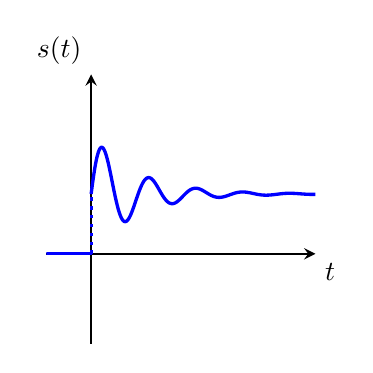
\begin{tikzpicture}
        \begin{axis}[
        axis line style = thick,
	ticks=none,
        height=5cm,
        width=5cm,
        axis x line=center,
        axis y line=center,
        xmin=-2,
        xmax=10,
        ymin=-1.5,
        ymax=3.0,
        xlabel={$t$},
        ylabel={$s(t)$},
        xlabel style={below right},
        ylabel style={above left},
        ]
        \addplot [very thick,color=blue,domain=-2:0, samples=101,unbounded coords=jump]{0};                                
	\addplot [very thick,color=blue,domain=0:10, samples=501,unbounded coords=jump]{sin(3*deg(x))*exp(-0.5*x)+1};
        \draw[dotted,very thick,blue] (axis cs:0,0) -- (axis cs:0,1); 
        \end{axis}
    \end{tikzpicture}

%\caption{Exemple d'}
\end{figure}
\setlength\intextsep{0pt}
}
Pour un signal en entrée, le temps $t=0$ permet de 
définir une origine des temps.
%\paragraph{Stable}

%\begin{center}
%\tikzsetnextfilename{stable-chap0_ext}
%\begin{tikzpicture}
	\begin{axis}
	[	ticks=none,
        axis line style = thick,
        height=5cm,
        width=5cm,
        axis x line=center,
        axis y line=center,
        xmin=-2,
        xmax=10,
        ymin=-1.5,
        ymax=3.0,
        xlabel={$t$},
        ylabel={$s(t)$},
        xlabel style={below right},
        ylabel style={above left},
	]
	\addplot[signalb,domain=-2:0] {0};
	\addplot[signalb,domain=0:10] {sin(3*deg(x))*exp(-x)+1};
	\draw[dotted,very thick,col1] (axis cs:0,0) -- (axis cs:0,1);
	\end{axis}
\end{tikzpicture}

%\end{center}                

%\begin{center}
%\tikzsetnextfilename{stable2-chap0_ext}
%    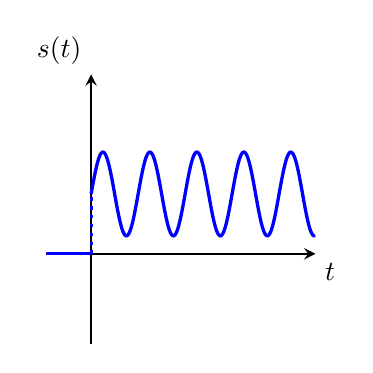
\begin{tikzpicture}
        \begin{axis}[
	ticks=none,
        axis line style = thick,
        height=5cm,
        width=5cm,
        axis x line=center,
        axis y line=center,
        xmin=-2,
        xmax=10,
        ymin=-1.5,
        ymax=3.0,
        xlabel={$t$},
        ylabel={$s(t)$},
        xlabel style={below right},
        ylabel style={above left},
        ]                                                                                                                     
        \addplot [very thick,color=blue,domain=-2:0, samples=101]{0};
	\addplot [very thick,color=blue,domain=0:10, samples=501]{0.7*sin(3*deg(x))+1};
	\draw[dotted,very thick,blue] (axis cs:0,0) -- (axis cs:0,1);
        \end{axis}
    \end{tikzpicture}

%\end{center}

%\begin{center}
%\tikzsetnextfilename{instable-chap0_ext}
%    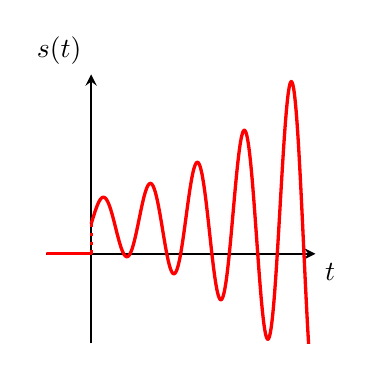
\begin{tikzpicture}
        \begin{axis}[
	ticks=none,
        axis line style = thick,
        height=5cm,
        width=5cm,
        axis x line=center,
        axis y line=center,
        xmin=-2,
        xmax=10,
        ymin=-3,
        ymax=6.0,
        xlabel={$t$},
        ylabel={$s(t)$},
        xlabel style={below right},
        ylabel style={above left},
        ]
        \addplot [very thick,color=red,domain=-2:0, samples=101,unbounded coords=jump]{0};
	\addplot [very thick,color=red,domain=0:10, samples=501,unbounded coords=jump]{0.8*sin(3*deg(x))*exp(0.2*x)+1};
	\draw[dotted,very thick,red] (axis cs:0,0) -- (axis cs:0,1);
        \end{axis}
    \end{tikzpicture}

%\end{center}

\paragraph{Retardé}
Un signal $s(t-\tau)$ est dit \textbf{retardé} d'un temps $\tau$ 
par rapport à $s(t)$, si on lui a fait subir un changement
d'origine des temps par rapport au signal $s(t)$.
\begin{center}
\tikzsetnextfilename{retarde-chap0_ext}
\begin{tikzpicture}
    \begin{axis}
    [   name=ax2,
        axis line style = thick,
        height=4cm,
        width=5cm,
        axis x line=center,
        axis y line=center,
        xmin=-2,
        xmax=6,
        ymin=-0.5,
        ymax=1.5,
        ytick={1},
        yticklabels={$1$},
        xtick=\empty,
        xlabel={$t$},
        ylabel={$s(t)$},
        xlabel style={below right},
        ylabel style={above left},
    ]
    \addplot [ultra thick,col1,domain=-2:0, samples=101]{0};
    \addplot [ultra thick,col1,domain=0:16, samples=101]{1-exp(-x)};
    \end{axis}
    \begin{axis}
    [   at={(ax2.south east)},
        xshift=4em,
        ytick=\empty,
        axis line style = thick,
        height=4cm,
        width=5cm,
        axis x line=center,
        axis y line=center,
        xmin=-2,
        xmax=6,
        ymin=-0.5,
        ymax=1.5,
        ytick={1},
        yticklabels={$1$},
        xlabel={$t$},
        ylabel={$s(t-\tau)$},
        xlabel style={below right},
        ylabel style={above left},
	xticklabels={$\tau$},
        xtick={2},
    ]
    \addplot [ultra thick,col1,domain=-2:2, samples=101]{0};
    \addplot [ultra thick,col1,domain=2:16, samples=101]{1-exp(-(x-2))};
    \end{axis}
\end{tikzpicture}

\end{center}

\paragraph{Périodique}
                                                                                                                              
Un signal est dit \textbf{périodique} s'il se reproduit identique à lui
même au bout d'un même intervalle de temps ou periode $T$. On définit alors sa fréquence $f$
qui est l'inverse de la période $f=1/T$ ou la pulsation $\omega$ définit par rapport au cercle unité
$\omega=2\pi f$.
{
\begin{figure}[!htb]
\centering
\tikzsetnextfilename{periodique-chap0_ext}
    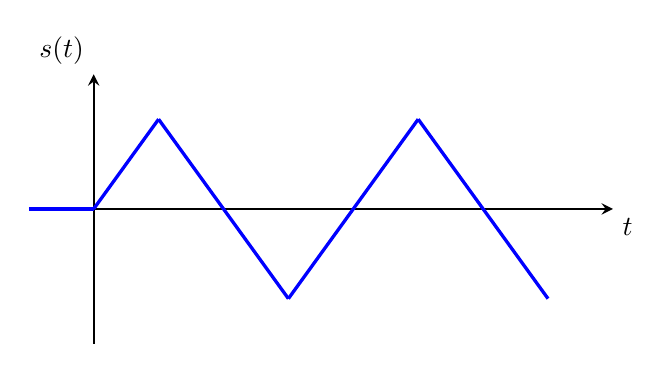
\begin{tikzpicture}
        \begin{axis}[
	ticks=none,
        axis line style = thick,
        height=5cm,
        width=9cm,
        axis x line=center,
        axis y line=center,
        xmin=-2,
        xmax=16,
        ymin=-1.5,
        ymax=1.5,
        xlabel={$t$},
        ylabel={$s(t)$},
        xlabel style={below right},
        ylabel style={above left},
        ]
        \addplot [very thick,color=blue,domain=-2:0, samples=101,unbounded coords=jump]{0};
        \addplot [very thick,color=blue,domain=0:2, samples=101,unbounded coords=jump]{0.5*x};
        \addplot [very thick,color=blue,domain=2:6, samples=101,unbounded coords=jump]{-0.5*x+2};
        \addplot [very thick,color=blue,domain=6:10, samples=101,unbounded coords=jump]{0.5*x-4};
        \addplot [very thick,color=blue,domain=10:14, samples=101,unbounded coords=jump]{-0.5*x+6};
        \end{axis}
    \end{tikzpicture}

\end{figure}
\setlength\intextsep{0pt}
}
                                                                                                                              
Le signal complet peut être totalement d'écrit en considérant un motif de base $s_0(t)$ telle que
\begin{align*}
s_0(t) =
\begin{dcases}
    s(t)&\quad\text{pour}\quad 0\le t\le T   \\
    0&\quad\text{pour}\quad t>T
\end{dcases}
\end{align*}
Le signal $s(t)$ est alors la somme (série) du motif retardé de $nT$ 
avec $n\in\mathbb{N}$ tel que :
$$
s(t)=\sum_0^\infty s_0(t-nT)
$$
L'analyse de Fourier est un outil fondamentale pour l'étude 
de ces signaux périodiques. Elle sort cependant légérement du cadre de ce cours.

%\clearpage
%%%%%%%%%%%%%%%%%%%%%%%%%%%%%%%%%%%%%%%%%%%%%%%%%%%%%%%%%%%%%%%%%
\subsection{Signaux usuels rencontrés\ldots\label{sec-signaux_usuels}}
%%%%%%%%%%%%%%%%%%%%%%%%%%%%%%%%%%%%%%%%%%%%%%%%%%%%%%%%%%%%%%%%

%Nous aurons l'occasion de rencontrer de nombreuses fois certains signaux.
Certains signaux sont des briques de base pour la construction de
signaux plus complexes. Il est alors essentiel de bien les caractériser.
Ici, nous distingons les signaux généralement utilisés en 
entrée des signaux généralement rencontrées en sortie des \gls{slci}.

\subsubsection{\ldots en entrée}

%%%%%%%%%%%%%%%%%%%%%%%%%%%%%%%%%%%%%%%%%%%%%%%%%%%%%%%%%%%%%%%%%%%%%
\paragraph{Impulsion de Dirac}
%%%%%%%%%%%%%%%%%%%%%%%%%%%%%%%%%%%%%%%%%%%%%%%%%%%%%%%%%%%%%%%%%%%%

L'impulsion de Dirac\footnote{\index{Dirac, Paul}Paul Dirac, (1902-1984) mathématicien et 
physicien britannique} $\delta(t)$ est une \og fonction\fg 
\footnote{Les guillemets sont essentiels pour ne pas se fâcher avec nos collègues mathématiciens.} telle que
\begin{align*}
\delta(t) : 
\begin{dcases}
	\int\limits_{-\infty}^{+\infty}	 \delta(t)\,\,\dd{t}&=1   \\
\int\limits_{-\infty}^{+\infty}  \delta(t)f(t)\,\,\dd{t}&=f(0)	
\end{dcases}
\end{align*}

C'est fonction est donc nulle partout sauf en $t=0$ où elle prend 
une valeur infinie. C'est pourquoi l'intégrale sur tous les nombres réels d'une impulsion 
de Dirac est normalisée à 1.
Graphiquement une impulsion de Dirac $\delta(t)$ est 
représentée par une flèche en $t=0$. La figure ci-dessous présente 
une impulsion de Dirac ainsi qu'une 
impulsion retardée de $\tau$ noté $\delta(t-\tau)$.

\begin{figure}[!h]
\begin{center}
\tikzsetnextfilename{dirac-chap0_ext}
\begin{tikzpicture}
    \begin{axis}
    [   name=ax0,
        ticks=none,
        axis line style = thick,
        height=5cm,
        width=5cm,
        axis x line=center,
        axis y line=center,
        xmin=-4,
        xmax=4,
        ymin=-1.5,
        ymax=3.0,
        xlabel={$t$},
        ylabel={$\delta(t)$},
        xlabel style={below right},
        ylabel style={above left},
    ]
    \draw[ultra thick,blue,-latex] (axis cs:0,0) -- (axis cs:0,2.0);
    \end{axis}
    \begin{axis}
    [   at={(ax0.south east)}, 
        xshift=4        em,                
        axis line style = thick,
        height=5cm,
        width=5cm,
        axis x line=center,
        axis y line=center,
        xmin=-4,
        xmax=4,
        ymin=-1.5,
        ymax=3.0,
        xlabel={$t$},
        ylabel={$\delta(t-\tau)$},
        xlabel style={below right},
        ylabel style={above left},
        xtick={2},
        xticklabels={$\tau$},
        ytick={10},
        yticklabels={},
    ]
    \draw[ultra thick,blue,-latex] (axis cs:2,0) -- (axis cs:2,2.0);
    \end{axis}
\end{tikzpicture}

\end{center}
%\caption{\label{fig-dirac}}
\end{figure}

L'impulsion de Dirac est expérimentalement approchée par un signal 
bref et de grande amplitude. Il est possible de montrer que la fonction
suivante $\delta_a(t)$ est une impulsion de Dirac lorsque $a\to0$.

Nous la rencontrerons quelque fois sous sa forme généralisée, 
$$
e(t)=E_0\delta(t)
$$
où $e(t)$ est le signal d'entrée du système et $E_0$ la valeur de l'amplitude de l'impulsion de Dirac
dont l'unité dépend de la nature du problème considéré.
\begin{figure}[!h]
\begin{center}
\tikzsetnextfilename{dirac_reel-chap0_ext}
\begin{tikzpicture}
    \begin{axis}
    [   ticks=none,
        axis line style = thick,
        height=5cm,
        width=5cm,
        axis x line=center,
        axis y line=center,
        xmin=-2,
        xmax=6,
        ymin=-1.5,
        ymax=3.0,
        xlabel={$t$},
        ylabel={$\delta_a(t)$},
        xlabel style={below right},
        ylabel style={above left}
    ]
    \addplot [signal,domain=-2:0] {0};
    \addplot [signal,domain=0:2 ] {2};
    \addplot [signal,domain=2:5 ] {0};
    \draw[dotted,very thick,blue] (axis cs:0,0) -- (axis cs:0,2);
    \draw[dotted,very thick,blue] (axis cs:2,2) -- (axis cs:2,0);
    \node[blue] at (axis cs:2,-0.5) {$a$};
    \node[blue] at (axis cs:-0.5,2) {$\dfrac{1}{a}$};
    \end{axis}
\end{tikzpicture}

    \caption{Représentation de l'impulsion de Dirac approchée. 
    Celle-ci tend vers l'impulsion de Dirac pour $a\to0$. On remarquera que l'aire du rectangle est toujours égale à 1.\label{fig-dirac2}}
\end{center}
\end{figure}

La réponse d'un système à une impulsion de Dirac est appelée \textbf{réponse impulsionnelle}.

Dans la pratique, une telle sollicitation breve et de grande amplitude
permet de parfaitement caractériser le système. La réponse impulsionnelle, qui en résulte, contient
toute l'information du système linéaire qui l'a élaboré.

%%%%%%%%%%%%%%%%%%%%%%%%%%%%%%%%%%%%%%%%%%%%%%%%%%%%%%%%%%%%%%%%%%%%%%
\paragraph{\'Echelon-unité}
%%%%%%%%%%%%%%%%%%%%%%%%%%%%%%%%%%%%%%%%%%%%%%%%%%%%%%%%%%%%%%%%%%%%%%

L'échelon-unité est défini par la fonction, noté $u(t)$, telle que :
$$
u(t)=
\begin{cases} 
0 \qquad \forall t<0    \\ 
1 \qquad \forall t\geq 0 
\end{cases}
$$

Cette fonction présente une marche\footnote{Nos 
collègues anglo-saxons l'appelle la \og\emph{step function}\fg} à $t=0$. 
Ci dessous nous la représentons avec la fonction retardée $u(t-\tau)$.
\begin{figure}[!h]
\begin{center}
\tikzsetnextfilename{echelon-chap0_ext}
\begin{tikzpicture}
    \begin{axis}
    [   name=ax2,
        axis line style = thick,
        height=5cm,
        width=5cm,
        axis x line=center,
        axis y line=center,
        xmin=-2,
        xmax=6,
        ymin=-1.5,
        ymax=1.5,
        ytick={1},
        yticklabels={$1$},
        xtick=\empty,
        xlabel={$t$},
        ylabel={$u(t)$},
        xlabel style={below right},
        ylabel style={above left},
    ]
    \addplot [signalb,domain=-2:0]{0};
    \addplot [signalb,domain=0:16]{1};
    \draw[dotted,very thick,blue] (axis cs:0,0) -- (axis cs:0,1);
    \end{axis}
    \begin{axis}
    [   at={(ax2.south east)},
        xshift=4em,
        ytick=\empty,
        axis line style = thick,
        height=5cm,
        width=5cm,
        axis x line=center,
        axis y line=center,
        xmin=-2,
        xmax=6,
        ymin=-1.5,
        ymax=1.5,
        ytick={1},
        yticklabels={$1$},
        xlabel={$t$},
        ylabel={$u(t-\tau)$},
        xlabel style={below right},
        ylabel style={above left},
	xticklabels={$\tau$},
        xtick={2},
    ]
    \addplot [signalb,domain=-2:2] {0};
    \addplot [signalb,domain=2:16] {1};
    \draw[dotted,very thick,blue] (axis cs:2,0) -- (axis cs:2,1);
    \end{axis}
\end{tikzpicture}

\end{center}
    \caption{Représentation graphique de (gauche) la fonction échelon-unité et (droite) la fonction 
    échelon-unité retardée de $\tau$\label{fig-echelon}}
\end{figure}

En général, l'échelon-unité est utilisé en entrée de nos systèmes pour 
modéliser des états fermé/ouvert (\og on/off\fg) ou encore en régulation.
Nous la rencontrerons souvent sous sa forme généralisée, 
$$
e(t)=E_0u(t)
$$
où $e(t)$ est le signal d'entrée du système et $E_0$ la valeur seuil de l'échelon dont 
l'unité dépend de la nature du problème considéré.

D'après les propriétés du signal échelon-unité et de la causalité, il est possible 
de rendre causale une fonction quelconque en la multipliant par un échélon-unité.

La réponse d'un système à un échelon est appelée \textbf{réponse indicielle}.

Remarquons que la fonction échelon-unité est l'intégrale de la distribution de Dirac,
$$
u(t)=\int\limits_{-\infty}^{t} \delta(\tau)\,\,\dd{\tau}
$$

%%%%%%%%%%%%%%%%%%%%%%%%%%%%%%%%%%%%%%%%%%%%%%%%%%%%%%%%%%%%%%%%%%%%%%
\paragraph{Rampe-unité}
%%%%%%%%%%%%%%%%%%%%%%%%%%%%%%%%%%%%%%%%%%%%%%%%%%%%%%%%%%%%%%%%%%%%%%

Le signal rampe-unité\footnote{On retrouve parfois~\cite{sueurautomatique} le terme 
d'échelon vitesse pour désigner la fonction rampe} est modélisé par la fonction $r(t)$ telle que :
$$
r(t)=
\begin{cases}
	0\,\,\,\,t<0 \\
	t\,\,\,\,t\geq0 
\end{cases}
$$
ou autrement dit, en utilisant la propriété de causalité de l'échelon:
$$
r(t)=t\cdot u(t)
$$

\begin{figure}[!h]
\begin{center}
\tikzsetnextfilename{rampe-chap0_ext}
    \begin{tikzpicture}
        \begin{axis}[
        name=ax2,
        ticks=none,
        axis line style = thick,
        height=5cm,
        width=5cm,
        axis x line=center,
        axis y line=center,
        xmin=-2,
        xmax=6,
        ymin=-1.5,
        ymax=6,
        xlabel={$t$},
        ylabel={$r(t)$},
        xlabel style={below right},
        ylabel style={above left},
        ]
        \addplot [ultra thick,color=blue,domain=-2:0, samples=101,unbounded coords=jump]{0};
        \addplot [ultra thick,color=blue,domain=0:15, samples=101,unbounded coords=jump]{x};
        \end{axis}
        \begin{axis}[
        at={(ax2.south east)},
        xshift=4em,
        %ticks=none,
        axis line style = thick,
        height=5cm,
        width=5cm,
        axis x line=center,
        axis y line=center,
        xmin=-2,
        xmax=8,
        ymin=-1.5,
        ymax=8,
        xlabel={$t$},
        ylabel={$r(t-\tau)$},
        xlabel style={below right},
        ylabel style={above left},
        xticklabels={$\tau$},
        xtick={2},

        ]
        \addplot [ultra thick,color=blue,domain=-2:2, samples=101,unbounded coords=jump]{0};
        \addplot [ultra thick,color=blue,domain=2:17, samples=101,unbounded coords=jump]{x-2};
        \end{axis}
    \end{tikzpicture}

\end{center}
    \caption{Représentation graphique de (gauche) la fonction rampe-unité et (droite) la fonction
        rampe-unité retardée de $\tau$\label{fig-rampe}}
\end{figure}
Remarquons que la fonction rampe est l'intégrale de l'échelon-unité, notamment 
$$
r(t)=\int\limits_{-\infty}^{t} u(\tau)\,\,\dd{\tau}
$$
La réponse d'un système à une rampe ne possède pas de nom spécifique, 
utilisé pour la distinguer des autres réponses. On parlera donc simplement 
de \textbf{réponse à une rampe}. 
%%%%%%%%%%%%%%%%%%%%%%%%%%%%%%%%%%%%%%%%%%%%%%%%%%%%%%%%%%%%%%%%%%%%%
\paragraph{Sinuso\"ide}
%%%%%%%%%%%%%%%%%%%%%%%%%%%%%%%%%%%%%%%%%%%%%%%%%%%%%%%%%%%%%%%%%%%%%
Le signal périodique sinuso\"idale $s(t)$ est la fonction telle que :
$$
s(t)=A\sin{(\omega t +\phi)}\cdot u(t)
$$
avec $A$ son amplitude, $\omega$ sa pulsation (en rad/s) et $\phi$ sa phase (rad).
%La pulsation permet de définir la fréquence $f=\dfrac{\omega}{2\pi}$ en \si{\hertz},  
%elle même liée à la période $T=\dfrac{1}{f}$ en \si{\second}.
\begin{figure}[!h]
\begin{center}
\tikzsetnextfilename{sinusoide-chap0-ext}
\begin{tikzpicture}
    \begin{axis}
    [   axis line style = thick,
        clip=false,
        height=5cm,
        width=10cm,
        axis x line=center,
        axis y line=center,
        xmin=-2,
        xmax=4*pi,
        ymin=-1.5,
        ymax=1.5,
        xlabel={$t$},
        ylabel={$s(t)$},
        xlabel style={below right},
        ylabel style={above left},
        ytick={-1,1},
        yticklabels={$-A$,$A$},
        xtick={},
        xticklabels={},
    ]
    \addplot[signalb,domain=-2:0]    {0};
    \addplot[signalb,domain=0:4*pi]  {sin(deg(x))};
    \addplot[signalr,domain=0:4*pi]  {sin(deg(x-pi*0.5))};
    \draw[blue] (axis cs:pi*0.5,1) -- (axis cs:pi*0.5,1.25);
    \draw[blue] (axis cs:pi*2.5,1) -- (axis cs:pi*2.5,1.25);
    \draw[blue,ultra thick, latex-latex] (axis cs:pi*0.5,1.2) -- 
    node[above,yshift=+0.2em]{$\dfrac{2\pi}{\omega}$} (axis cs:pi*2.5,1.2);
    \draw[blue] (axis cs:pi*1.5,-1) -- (axis cs:pi*1.5,-1.25);
    \draw[blue] (axis cs:pi*1.5+pi*0.5,-1) -- (axis cs:pi*1.5+pi*0.5,-1.25);
    \draw[blue,ultra thick, latex-latex] (axis cs:pi*1.5,-1.2) --
    node[below,yshift=-0.2em]{$\dfrac{\Delta\phi}{\omega}$}
    (axis cs:pi*1.5+pi*0.5,-1.2);
    \end{axis}
\end{tikzpicture}

\end{center}
    \caption{Représentation de signaux sinuso\"idaux de même pulsation et même amplitude. 
    (bleu) de phase $\phi=0$ et (rouge) de phase $\phi=-\dfrac{\pi}{2}$.\label{fig-sin}}
\end{figure}


\begin{table}[!h]
\centering
\begin{tabular}{C{2cm}C{4cm}C{9cm}N}
\hhline{====}
    Déphasage               & Terminologie                  & Graphe &  \\[1em]
\hhline{====}
$\Delta\phi=0$              & \og en phase\fg               & \tikzsetnextfilename{sinusoide_enp-chap0-ext}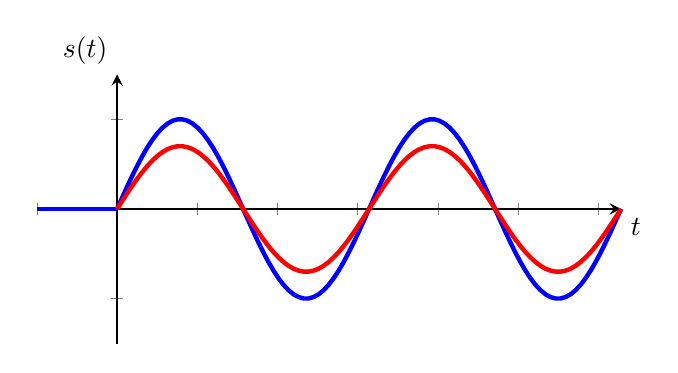
\begin{tikzpicture}
\begin{axis}[
        axis line style = thick,
        clip=false,
        height=5cm,
        width=9cm,
        axis x line=center,
        axis y line=center,
        xmin=-2,
        xmax=4*pi,
        ymin=-1.5,
        ymax=1.5,
        xlabel={$t$},
        ylabel={$s(t)$},
        xlabel style={below right},
        ylabel style={above left},
        ytick={-1,1},
        yticklabels={},
        xtick={},
        xticklabels={},
        ]

            \addplot [ultra thick,color=blue,domain=-2:0, samples=101]{0};
            \addplot [ultra thick,color=blue,domain=0:4*pi, samples=101]{sin(deg(x))};
            \addplot [ultra thick,color=red,domain=0:4*pi, samples=101]{0.7*sin(deg(x))};
        \end{axis}
\end{tikzpicture}
 & \\[5em]
\hhline{----}
$\Delta\phi=\pm\pi$         & \og en opposition de phase\fg & \tikzsetnextfilename{sinusoide_enop-chap0-ext}\begin{tikzpicture}
    \begin{axis}
    [	axis line style = thick,
        clip=false,
        height=5cm,
        width=9cm,
        axis x line=center,
        axis y line=center,
        xmin=-2,
        xmax=4*pi,
        ymin=-1.5,
        ymax=1.5,
        xlabel={$t$},
        ylabel={$s(t)$},
        xlabel style={below right},
        ylabel style={above left},
        ytick={-1,1},
        yticklabels={},
        xtick={},
        xticklabels={},
    ]
    \addplot[signal,domain=-2:0]{0};
    \addplot[signal,blue,domain=0:4*pi]{sin(deg(x))};
    \addplot[signal,red,domain=0:4*pi]{0.7*sin(deg(x-pi))};
    \end{axis}
\end{tikzpicture}
 & \\
\hhline{----}
    $\Delta\phi=-\dfrac{\pi}{2}$ & \og en quadrature de phase\fg (retard de phase) & \tikzsetnextfilename{sinusoide_enqp-chap0-ext}\begin{tikzpicture}
    \begin{axis}
    [	axis line style = thick,
        clip=false,
        height=5cm,
        width=9cm,
        axis x line=center,
        axis y line=center,
        xmin=-2,
        xmax=4*pi,
        ymin=-1.5,
        ymax=1.5,
        xlabel={$t$},
        ylabel={$s(t)$},
        xlabel style={below right},
        ylabel style={above left},
        ytick={-1,1},
        yticklabels={},
        xtick={},
        xticklabels={},
    ]
    \addplot[signalb,domain=-2:0]   {0};
    \addplot[signalb,domain=0:4*pi] {sin(deg(x))};
    \addplot[signalr,domain=0:4*pi] {0.7*sin(deg(x-pi*0.5))};
    \end{axis}
\end{tikzpicture}
 & \\
\hhline{----}
    $\Delta\phi=\dfrac{\pi}{2}$ & \og en quadrature de phase\fg (avance de phase) & \tikzsetnextfilename{sinusoide_enqp2-chap0-ext}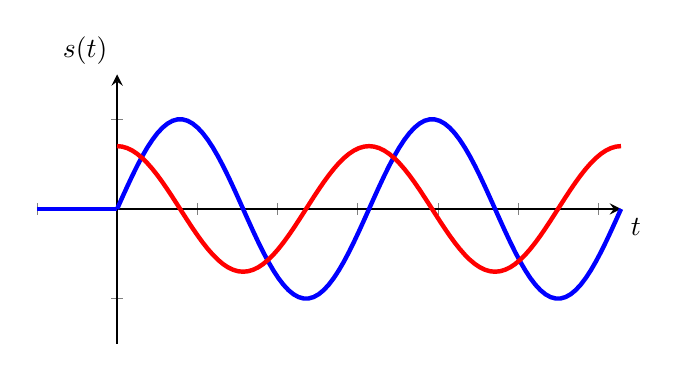
\begin{tikzpicture}
\begin{axis}[
        axis line style = thick,
        clip=false,
        height=5cm,
        width=9cm,
        axis x line=center,
        axis y line=center,
        xmin=-2,
        xmax=4*pi,
        ymin=-1.5,
        ymax=1.5,
        xlabel={$t$},
        ylabel={$s(t)$},
        xlabel style={below right},
        ylabel style={above left},
        ytick={-1,1},
        yticklabels={},
        xtick={},
        xticklabels={},
        ]

            \addplot [ultra thick,color=blue,domain=-2:0, samples=101]{0};
            \addplot [ultra thick,color=blue,domain=0:4*pi, samples=101]{sin(deg(x))};
            \addplot [ultra thick,color=red,domain=0:4*pi, samples=101]{0.7*sin(deg(x+pi*0.5))};
        %    \draw[blue,] (axis cs:pi*0.5,1) -- (axis cs:pi*0.5,1.25);
        %    \draw[blue] (axis cs:pi*2.5,1) -- (axis cs:pi*2.5,1.25);
        %    \draw[blue,ultra thick, latex-latex] (axis cs:pi*0.5,1.2) --node[above,yshift=+0.2em]{$\dfrac{2\pi}{\omega}$} (axis cs:pi*2.5,1.2);
        %    \draw[blue,] (axis cs:pi*1.5,-1) -- (axis cs:pi*1.5,-1.25);
        %    \draw[blue] (axis cs:pi*1.5+pi*0.5,-1) -- (axis cs:pi*1.5+pi*0.5,-1.25);
        %    \draw[blue,ultra thick, latex-latex] (axis cs:pi*1.5,-1.2) --node[below,yshift=-0.2em]{$\dfrac{\Delta\phi}{\omega}$} (axis cs:pi*1.5+pi*0.5,-1.2);
        \end{axis}
\end{tikzpicture}
 & \\
\hhline{====}
\end{tabular}
\caption{Différents types de déphasage d'un (rouge) signal sinusoidal $s_2(t)$ par rapport à (bleu) 
         un signal de référence $s_1(t)$ de phase nulle.\label{tab-sin_deph}}
\end{table}

La réponse d'un système à une sinuso\"ide est appelée la \textbf{réponse harmonique}
et son analyse fera l'objet de tout un chapitre (\Cref{chap-anafreq}).

Le~\cref{tab-sin_deph} rappel la terminologie associé au déphasage entre 
deux signaux sinuso\"idaux. 

\clearpage
\subsubsection{\ldots en sortie}
%%%%%%%%%%%%%%%%%%%%%%%%%%%%%%%%%%%%%%%%%%%%%%%%%%%%%%%%%%%%%%%%%%%%%%
\paragraph{Exponentielle décroissante}
%%%%%%%%%%%%%%%%%%%%%%%%%%%%%%%%%%%%%%%%%%%%%%%%%%%%%%%%%%%%%%%%%%%%%%
La fonction exponentielle décroissante $s(t)$ est telle que :
$$
s(t)=e^{-at}\cdot u(t)
$$  
avec $a$ l'inverse d'un temps caractéristique d'un amortissement.
Cette fonction tend vers 0 pour tout $a>0$ à $t\rightarrow\infty$ et diverge pour $a<0$
\begin{figure}[!h]
\begin{center}
\tikzsetnextfilename{exp_dec-chap0_ext}
    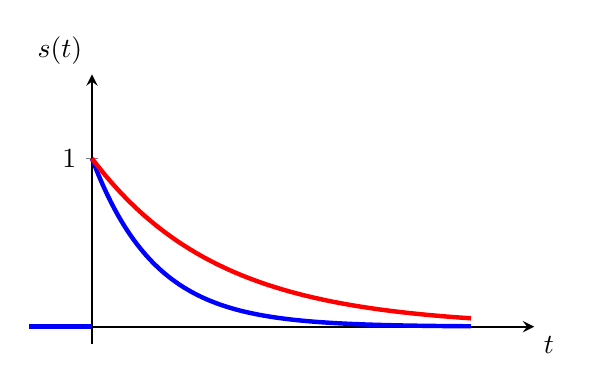
\begin{tikzpicture}
        \begin{axis}[
        axis line style = thick,
%        clip=false,
        height=5cm,
        width=8cm,
        axis x line=center,
        axis y line=center,
        xmin=-1,
        xmax=7,
        ymin=-0.1,
        ymax=1.5,
        xlabel={$t$},
        ylabel={$s(t)$},
        xlabel style={below right},
        ylabel style={above left},
        ytick={1},
        yticklabels={$1$},
        xtick=\empty,
        ]
            \addplot [ultra thick,color=blue,domain=-1:0, samples=101,unbounded coords=jump]{0};
            \addplot [ultra thick,color=blue,domain=0:6, samples=101,unbounded coords=jump]{exp(-x)};
            \addplot [ultra thick,color=red,domain=0:6, samples=101,unbounded coords=jump] {exp(-0.5*x)};
        \end{axis}
    \end{tikzpicture}

\end{center}
    \caption{Représentation de la fonction exponentielle pour 
             différentes valeurs du paramètre $a$.\label{fig-exp}}
\end{figure}


%%%%%%%%%%%%%%%%%%%%%%%%%%%%%%%%%%%%%%%%%%%%%%%%%%%%%%%%%%%%%%%%%%%%%
\paragraph{Sinuso\"ide amortie}
%%%%%%%%%%%%%%%%%%%%%%%%%%%%%%%%%%%%%%%%%%%%%%%%%%%%%%%%%%%%%%%%%%%%%
La fonction sinuso\"idale amortie $s(t)$ est la fonction telle que :
$$
s(t)=Ae^{-at}\sin{(\omega t +\phi)}\cdot u(t)
$$
%où $a>0$ est l'inverse d'un temps caractéristique de l'amortissement.
Cette fonction est donc le produit d'une exponentielle décroissante et d'une sinuso\"ide.
\begin{figure}[!h]
\begin{center}
\tikzsetnextfilename{sinusoide_amortie-chap0-ext}
    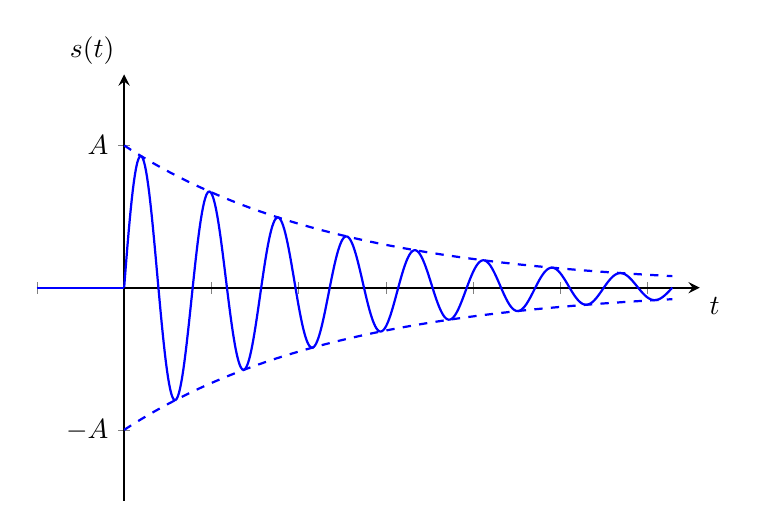
\begin{tikzpicture}
        \begin{axis}[
        axis line style = thick,
        clip=false,
        height=7cm,
        width=10cm,
        axis x line=center,
        axis y line=center,
        xmin=-2,
        xmax=4.2*pi,
        ymin=-1.5,
        ymax=1.5,
        xlabel={$t$},
        ylabel={$s(t)$},
        xlabel style={below right},
        ylabel style={above left},
        ytick={-1,1},
        yticklabels={$-A$,$A$},
        xtick={},
        xticklabels={},
        ]

            \addplot [thick,color=blue,domain=-2:0, samples=11,unbounded coords=jump]{0};
            \addplot [thick,color=blue,domain=0:4*pi, samples=501,unbounded coords=jump]{exp(-0.2*x)*sin(4*deg(x))};
            \addplot [dashed,thick,color=blue,domain=0:4*pi, samples=501,unbounded coords=jump]{exp(-0.2*x)};
            \addplot [dashed,thick,color=blue,domain=0:4*pi, samples=501,unbounded coords=jump]{-exp(-0.2*x)};
            %\addplot [thick,color=red,domain=0:4*pi, samples=501,unbounded coords=jump]{exp(-0.2*x)*sin(deg(4*x-pi*0.5))};
%            \draw[blue,] (axis cs:pi*0.5,1) -- (axis cs:pi*0.5,1.25);
%            \draw[blue] (axis cs:pi*2.5,1) -- (axis cs:pi*2.5,1.25);
%            \draw[blue,ultra thick, latex-latex] (axis cs:pi*0.5,1.2) --node[above,yshift=+0.2em]{$\dfrac{2\pi}{\omega}$} (axis cs:pi*2.5,1.2);
%            \draw[blue,] (axis cs:pi*1.5,-1) -- (axis cs:pi*1.5,-1.25);
%            \draw[blue] (axis cs:pi*1.5+pi*0.5,-1) -- (axis cs:pi*1.5+pi*0.5,-1.25);
%            \draw[blue,ultra thick, latex-latex] (axis cs:pi*1.5,-1.2) --node[below,yshift=-0.2em]{$\dfrac{\Delta\phi}{\omega}$} (axis cs:pi*1.5+pi*0.5,-1.2);
        \end{axis}
    \end{tikzpicture}

\end{center}
    \caption{Représentation d'un sinuso\"ide amortie. L'enveloppe en pointillé 
correspond aux fonctions $e^{-at}$ et $-e^{-at}$.\label{fig-sin_amor}}
\end{figure}


\clearpage
%%%%%%%%%%%%%%%%%%%%%%%%%%%%%%%%%%%%%%%%%%%%%%%%%%%%%%%%%%%%%%%%%
\section{La transformée de Laplace}
%%%%%%%%%%%%%%%%%%%%%%%%%%%%%%%%%%%%%%%%%%%%%%%%%%%%%%%%%%%%%%%%%
La transformée de Laplace\footnote{\index{Laplace, Pierre-Simon}Pierre-Simon de Laplace, (1749-1827) 
mathématicien, astronome, physicien et homme politique français} est l'outil indispensable 
pour l'étude des \gls{slci}. Celle-çi nous sera très utile pour 
la résolution des équations différentielles 
et nous permettra également de définir la notion de 
fonction de transfert reliant l'entrée et la sortie d'un système linéaire.



%%%%%%%%%%%%%%%%%%%%%%%%%%%%%%%%%%%%%%%%%%%%%%%%%%%%%%%%%%%%%%%%%
\subsection{Définition}
%%%%%%%%%%%%%%%%%%%%%%%%%%%%%%%%%%%%%%%%%%%%%%%%%%%%%%%%%%%%%%%%
La~\gls{tl}, notée $\mathscr{L}$, d'une fonction causale $s$ (pour signal) 
d'une variable réelle $t$ (pour temps), est la fonction $S$ 
de la variable complexe $p$, définie par :
\begin{bequation}[ams align]
S(p)=\laplace{s(t)}=\int_{0}^{+\infty} e^{-pt}s(t)\dd{t}.\label{eq-lap}
\end{bequation}


On dit également que \textbf{$S(p)$ est l'image dans le domaine de 
Laplace de la fonction $s(t)$ du domaine temporel.}
De plus la transformée $S(p)$ de $s(t)$ est unique et parfaitement définie. 
Connaissant $S(p)$ on en déduit $s(t)$
par la transformation inverse 
$$
s(t)=\laplacei{S(p)}
$$
%Les transformations inverses sont tabulées à l'\cref{annexe-lap}. 

Il existe une forme analytique de la transformée inverse basée sur
la formule de Mellin-Fourier\cite{Ostertag}:
$$
s(t)=\laplacei{S(p)}=\int_{c-j\infty}^{c+j\infty} e^{pt}S(p)\dd{p}
$$
L'intégration de celle-ci est difficile à mettre en oeuvre\footnote{
Il existe différentes méthodes numériques de transformée de Laplace inverse (\cref{annexe-invL}).
Ces méthodes, hors programme, peuvent cependant faire l'objet d'un projet numérique
intéressant.}, on préferera utilisé
les tables de transformations de Laplace pour réaliser la correspondance inverse (\cref{annexe-lap}).
Lorsque la transformation
n'existe pas dans les tables, il est possible de réaliser une décompostion en éléments 
simples de la réponse $S(p)$ pour se placer dans un cas usuel (\cref{annexe-DES}).

Remarquons, dès à présent l'utilisation d'une convention utile: 
\textbf{les fonctions du temps seront toujours désignées par une
minuscule, et les fonctions complexes par la majuscule respective}.

%%%%%%%%%%%%%%%%%%%%%%%%%%%%%%%%%%%%%%%%%%%%%%%%%%%%%%%%%%%%%%%%%%%%
\subsection{Propriétés}
%%%%%%%%%%%%%%%%%%%%%%%%%%%%%%%%%%%%%%%%%%%%%%%%%%%%%%%%%%%%%%%%%%%%
Nous allons ici uniquement présenter les principales propriétés de la TL, 
on se rapportera à nouveau à l'\cref{annexe-lap} pour 
une liste exhaustive de ces propriétés.

La propriété fondamentale de la transformée de Laplace est d'être linéaire.
%%%%%%%%%%%%%%%%%%%%%%%%%%%%%%%%%%%%%%%%%%%%%%%%%%%%%%%%%%%%%%%%%%%%
\paragraph{Linéarité}
%%%%%%%%%%%%%%%%%%%%%%%%%%%%%%%%%%%%%%%%%%%%%%%%%%%%%%%%%%%%%%%%%%%%
Soit deux signaux $s_1(t)$ et $s_2(t)$ continus et $S_1(p)$ et $S_2(p)$ leurs
transformées de Laplace respectives. La transformée de Laplace d'une 
relation linéaire quelconque de $s_1(t)$ et $s_2(t)$ est une relation linéaire 
de $S_1(p)$ et $S_2(p)$. Autrement dit,
\begin{bequation}[ams align]
	\laplace{as_1(t)+bs_2(t)}=aS_1(p)+bS_2(p)
\end{bequation}

%%%%%%%%%%%%%%%%%%%%%%%%%%%%%%%%%%%%%%%%%%%%%%%%%%%%%%%%%%%%%%%%%%%%
\paragraph{Retard en $t$ (temporel)}
%%%%%%%%%%%%%%%%%%%%%%%%%%%%%%%%%%%%%%%%%%%%%%%%%%%%%%%%%%%%%%%%%%%%
Soit $s(t-\tau)$ un signal $s(t)$ présentant un retard $\tau$.
$$
\laplace{s(t-\tau)}=\int_{0}^{+\infty} e^{-pt}s(t-\tau)\dd{t}
$$
en appliquant le changement de variable $t'=t-\tau$, on obtient $t=t'+\tau$ et $\dd{t}=\dd{t}$
$$
\laplace{s(t-\tau)}=\int_{\tau}^{+\infty} e^{-p(t'+\tau)}s(t')\dd{t'}=e^{-p\tau}\int_{0}^{+\infty} e^{-pt'}s(t')\dd{t'}
$$
on reconnaît dans cette dernière expression la définition de la transformée de Laplace, on écrit alors :
\begin{bequation}[ams align]
    \laplace{s(t-\tau)}=e^{-p\tau}S(p)
\end{bequation}
%%%%%%%%%%%%%%%%%%%%%%%%%%%%%%%%%%%%%%%%%%%%%%%%%%%%%%%%%%%%%%%%%%%%
\paragraph{Retard en $p$ (Thèorème de l'amortissement)}
%%%%%%%%%%%%%%%%%%%%%%%%%%%%%%%%%%%%%%%%%%%%%%%%%%%%%%%%%%%%%%%%%%%%
Soit $s(t)$ un signal de transformée de Laplace $S(p)$. La transformée 
de Laplace du signal modifié $e^{-at}s(t)$ s'écrit :
$$
\laplace{e^{-at}s(t)}=\int_{0}^{+\infty} e^{-pt}e^{-at}s(t)\dd{t}=\int_{0}^{+\infty} e^{-(p+a)t}s(t)\dd{t}
$$
on reconnaît dans cette dernière expression la définition de la transformée de Laplace pour $p+a$,
 on obtient donc la transformée,
\begin{bequation}[ams align]
    \laplace{e^{-at}s(t)}=S(p+a)
\end{bequation}
ou encore,
\begin{bequation}[ams align]
    \laplacei{S(p+a)}=e^{-at}s(t).
\end{bequation}


%%%%%%%%%%%%%%%%%%%%%%%%%%%%%%%%%%%%%%%%%%%%%%%%%%%%%%%%%%%%%%%%%%%
\paragraph{Dérivation}
%%%%%%%%%%%%%%%%%%%%%%%%%%%%%%%%%%%%%%%%%%%%%%%%%%%%%%%%%%%%%%%%%%%
Soit un signal $s(t)$ continu et dérivable pour $t\ge0$ et $S(p)$ sa transformée.
Par définition de la transformée de Laplace 
$$
\laplace{\devi{s(t)}{}}=\int_{0}^{+\infty} e^{-pt}\devi{s(t)}{}\dd{t}
$$
par intégration par parties
\begin{align*}
    v=e^{-pt}\qquad&\dd{u}=\devi{s(t)}{}\dd{t}\\
    \dd{v}=-pe^{-pt}\dd{t}\qquad&u=s(t)
\end{align*}
\begin{align*}
    \laplace{\devi{s(t)}{}}&=\left[s(t)e^{-pt}\right]_0^{+\infty}-p\int_{0}^{+\infty} e^{-pt}s(t)\dd{t} \\
                           &=-s(0)+pS(p)
\end{align*}
ou encore
\begin{bequation}[ams align]
    \laplace{\devi{s(t)}{}}=pS(p)-s(0)
\end{bequation}
On généralise à tous les ordres de dérivation dans le cas de conditions initiales nulles.
$$
\laplace{\devi{s(t)}{n}}=p^nS(p)
$$

Remarquons alors que \textbf{dériver dans le domaine temporel consiste à multiplier par 
$p$ dans le domaine de Laplace.}
%%%%%%%%%%%%%%%%%%%%%%%%%%%%%%%%%%%%%%%%%%%%%%%%%%%%%%%%%%%%%%%%%%%%
\paragraph{Intégration}
%%%%%%%%%%%%%%%%%%%%%%%%%%%%%%%%%%%%%%%%%%%%%%%%%%%%%%%%%%%%%%%%%%%%
Soient  des signaux $v(t)$ et $s(t)$ tel que $v(t)=\int_{0}^{t}s(\tau)\dd{\tau}$. 
Par définition,
$$
\laplace{v(t)}=\int_{0}^{+\infty} e^{-pt}v(t)\dd{t}
$$
par intégration par parties,
\begin{align*}
    v=v(t)\qquad&\dd{u}=e^{-pt}\dd{t}\\
    \dd{v}=s(t)\dd{t}\qquad&u=-\dfrac{1}{p}e^{-pt}
\end{align*} 
\begin{align*}
    \laplace{v(t)}&=\left[-\dfrac{1}{p}v(t)e^{-pt}\right]_0^{+\infty}-\int_{0}^{+\infty} -\dfrac{1}{p}e^{-pt}s(t)\dd{t} \\
    &=\dfrac{1}{p}\int_{0}^{+\infty} e^{-pt}s(t)\dd{t}+\dfrac{s(0)}{p}
\end{align*}
ou encore
\begin{bequation}[ams align]
    \laplace{\int_{0}^{t}s(\tau)\dd{\tau}}=\dfrac{S(p)}{p}+\dfrac{s(0)}{p}
\end{bequation}
Remarquons alors que \textbf{intégrer dans le domaine temporel consiste à diviser par $p$ 
dans le domaine de Laplace.}

%%%%%%%%%%%%%%%%%%%%%%%%%%%%%%%%%%%%%%%%%%%%%%%%%%%%%%%%%%%%%%%%%%%%%
\paragraph{Théorème de la valeur initiale}
%%%%%%%%%%%%%%%%%%%%%%%%%%%%%%%%%%%%%%%%%%%%%%%%%%%%%%%%%%%%%%%%%%%%%
\index{Théorème!de la valeur initiale}
\begin{bequation}[ams align]
    s(0)=\lim\limits_{p\rightarrow+\infty} p S(p)\qquad \forall S(p)
\end{bequation}
où $s(0)$ est la valeur d'un signal $s(t)$ pour $t=0$.
Ce théorème est utilisé pour déterminer la valeur initiale
dans le domaine temporelle d'un signal dont on connait 
uniquement la transformée de Laplace.

%%%%%%%%%%%%%%%%%%%%%%%%%%%%%%%%%%%%%%%%%%%%%%%%%%%%%%%%%%%%%%%%%%%%%
\paragraph{Théorème de la valeur finale}
%%%%%%%%%%%%%%%%%%%%%%%%%%%%%%%%%%%%%%%%%%%%%%%%%%%%%%%%%%%%%%%%%%%%%
\index{Théorème!de la valeur finale}
\begin{bequation}[ams align]
    s(\infty)=\lim\limits_{p\rightarrow0} p S(p)
\end{bequation}
où $s(\infty)$ est la valeur d'un signal $s(t)$ pour $t\to\infty$.
Ce théorème n'est valable que si $s(\infty)$ est définie. On dira plus tard
si le signal est stable.


%%%%%%%%%%%%%%%%%%%%%%%%%%%%%%%%%%%%%%%%%%%%%%%%%%%%%%%%%%%%%%%%%%%%%
\paragraph{Transformée de Laplace d'un produit de convolution}
%%%%%%%%%%%%%%%%%%%%%%%%%%%%%%%%%%%%%%%%%%%%%%%%%%%%%%%%%%%%%%%%%%%%%
Le produit de convolution de deux signaux $h(t)$ et $e(t)$ que l'on note $(h*e)(t)$
est défini par :
$$
(h*e)(t)=\int_{-\infty}^{+\infty}h(t-\tau)e(\tau)\dd{\tau}
$$
La transformée de Laplace transforme le produit de convolution en un simple
produit des signaux dans le domaine de Laplace. Formellement,
\begin{bequation}[ams align]
    \laplace{(h*e)(t)}=H(p)E(p)
\end{bequation}
Si cette propriété est fondamentale, nous ne l'utiliserons 
que très exceptionnellement. Nous la rencontrerons à nouveau 
lorsque nous introduierons la fonction de transfert d'un système linéaire.

%%%%%%%%%%%%%%%%%%%%%%%%%%%%%%%%%%%%%%%%%%%%%%%%%%%%%%%%%%%%%%%%%
\subsection{Transformées des signaux usuels}
%%%%%%%%%%%%%%%%%%%%%%%%%%%%%%%%%%%%%%%%%%%%%%%%%%%%%%%%%%%%%%%%%%
Nous présentons les transformées de Laplace des signaux usuels introduits
au paragraphe~\ref{sec-signaux_usuels}

%%%%%%%%%%%%%%%%%%%%%%%%%%%%%%%%%%%%%%%%%%%%%%%%%%%%%%%%%%%%%%%%%%
\paragraph{Transformée d'une impulsion de Dirac}
%%%%%%%%%%%%%%%%%%%%%%%%%%%%%%%%%%%%%%%%%%%%%%%%%%%%%%%%%%%%%%%%%
Par simple application des définitions 
de la~\gls{tl} et de l'impulsion de Dirac, la transformée d'une 
impulsion de Dirac $\delta(t)$ s'écrit:
$$
\laplace{\delta(t)}=\int_{0}^{+\infty} e^{-pt}\,\delta(t)\dd{t}=1
$$
ou encore
\begin{bequation}[ams align]
    \laplace{\delta(t)}=1
\end{bequation}

%%%%%%%%%%%%%%%%%%%%%%%%%%%%%%%%%%%%%%%%%%%%%%%%%%%%%%%%%%%%%%%%%%
\paragraph{Transformée d'un échelon-unité}
%%%%%%%%%%%%%%%%%%%%%%%%%%%%%%%%%%%%%%%%%%%%%%%%%%%%%%%%%%%%%%%%%%
La transformée de Laplace d'un signal échelon-unité  s'écrit : 
$$
\laplace{u(t)}=\int_{0}^{+\infty} e^{-pt}\,u(t)\dd{t}=\int_{0}^{+\infty} e^{-pt}\dd{t}=\left[\dfrac{-e^{-pt}}{p}\right]_0^{+\infty}=\dfrac{1}{p}
$$
ou encore
\begin{bequation}[ams align]
    \laplace{u(t)}=\dfrac{1}{p}
\end{bequation}
Dans le cas de la forme généralisée, il suffit de multiplier par une constante.

%%%%%%%%%%%%%%%%%%%%%%%%%%%%%%%%%%%%%%%%%%%%%%%%%%%%%%%%%%%%%%%%%%
\paragraph{Transformée d'une rampe}
%%%%%%%%%%%%%%%%%%%%%%%%%%%%%%%%%%%%%%%%%%%%%%%%%%%%%%%%%%%%%%%%%%
La transformée de Laplace d'un signal rampe s'écrit :
$$
\laplace{r(t)}=\int_{0}^{+\infty} e^{-pt}r(t)\dd{t}=\int_{0}^{+\infty} te^{-pt}\dd{t}
$$
Par intégration par parties:
\begin{align*}
    v=-\dfrac{1}{p}e^{-pt}\qquad&\dd{u}=\dd{t}\\
    \dd{v}=e^{-pt}\dd{t}\qquad&u=t
\end{align*}
$$
\int_{0}^{+\infty} te^{-pt}\dd{t} = \left[-t\dfrac{1}{p}e^{-pt}\right]_0^{+\infty}-\int_{0}^{+\infty} -\dfrac{1}{p}e^{-pt}\dd{t}=\dfrac{1}{p^2}
$$
ou encore
\begin{bequation}[ams align]
    \laplace{r(t)}=\laplace{t\cdot u(t)}=\dfrac{1}{p^2}.
\end{bequation}

On généralise aux ordres supérieures (parabolique,cubique\ldots) :
\begin{bequation}[ams align]
    \laplace{\dfrac{1}{n!}t^n\cdot u(t)}=\dfrac{1}{p^{n+1}}.
\end{bequation}


%%%%%%%%%%%%%%%%%%%%%%%%%%%%%%%%%%%%%%%%%%%%%%%%%%%%%%%%%%%%%%%%%%%%
\paragraph{Transformée d'une exponentielle décroissante}
%%%%%%%%%%%%%%%%%%%%%%%%%%%%%%%%%%%%%%%%%%%%%%%%%%%%%%%%%%%%%%%%%%%%
La transformée de Laplace d'une exponentielle décroissante s'écrit :
$$
\laplace{e^{-at}u(t)}=\int_{0}^{+\infty} e^{-pt}e^{-at}\dd{t}=\int_{0}^{+\infty} e^{-(p+a)t}\dd{t} = \dfrac{1}{p+a}
$$
ou encore
\begin{bequation}[ams align]
    \laplace{e^{-at}u(t)}=\dfrac{1}{p+a}
\end{bequation}
Nous aurions pu utiliser la propriété du retard en p (Théorème de 
l'amortissement) pour déterminer cette transformée de Laplace.


%%%%%%%%%%%%%%%%%%%%%%%%%%%%%%%%%%%%%%%%%%%%%%%%%%%%%%%%%%%%%%%%%%%%
\paragraph{Transformée d'un sinus}
%%%%%%%%%%%%%%%%%%%%%%%%%%%%%%%%%%%%%%%%%%%%%%%%%%%%%%%%%%%%%%%%%%%%
La transformée de Laplace d'un sinus s'écrit :
\begin{align*}
\laplace{\sin{\omega t}\cdot u(t)}&=\int_{0}^{+\infty}e^{-pt}\dfrac{e^{\jw t}-e^{-\jw t}}{2j}\dd{t}\\
&=\dfrac{1}{2j}\int_{0}^{+\infty}e^{-(p-\jw)t}\dd{t} - \dfrac{1}{2j}\int_{0}^{+\infty}e^{-(p+\jw)t}\dd{t} \\
&=\dfrac{1}{2j}\left( \dfrac{1}{p-\jw}-\dfrac{1}{p+\jw}\right)\\
&=\dfrac{\omega}{p^2+\omega^2}
\end{align*}
ou encore
\begin{bequation}[ams align]
    \laplace{\sin{\omega t}\cdot u(t)}=\dfrac{\omega}{p^2+\omega^2}
\end{bequation}

%%%%%%%%%%%%%%%%%%%%%%%%%%%%%%%%%%%%%%%%%%%%%%%%%%%%%%%%%%%%%%%%%%%%
\paragraph{Transformée d'un cosinus}
%%%%%%%%%%%%%%%%%%%%%%%%%%%%%%%%%%%%%%%%%%%%%%%%%%%%%%%%%%%%%%%%%%%%
La transformée de Laplace d'un cosinus s'écrit :
\begin{align*}
\laplace{\cos{\omega t}\cdot u(t)}&=\int_{0}^{+\infty}e^{-pt}\dfrac{e^{\jw t}+e^{-\jw t}}{2}\dd{t}\\
&=\dfrac{1}{2}\int_{0}^{+\infty}e^{-(p-\jw)t}\dd{t} + \dfrac{1}{2j}\int_{0}^{+\infty}e^{-(p+\jw)t}\dd{t} \\
&=\dfrac{1}{2}\left( \dfrac{1}{p-\jw}+\dfrac{1}{p+\jw}\right)\\
&=\dfrac{p}{p^2+\omega^2}
\end{align*}
ou encore
\begin{bequation}[ams align]
    \laplace{\cos{\omega t}\cdot u(t)}=\dfrac{p}{p^2+\omega^2}
\end{bequation}
%Exercice
%La même approche appliquée pour la fonction cosinus, nous donne :
%\begin{bequation}[ams align]
%    \laplace{\cos{\omega t}\cdot u(t)}=\dfrac{p}{p^2+\omega^2}
%\end{bequation}

%Exercice
%%%%%%%%%%%%%%%%%%%%%%%%%%%%%%%%%%%%%%%%%%%%%%%%%%%%%%%%%%%%%%%%%%%%
%\paragraph{Transformée d'une sinuso\"ide amortie}
%%%%%%%%%%%%%%%%%%%%%%%%%%%%%%%%%%%%%%%%%%%%%%%%%%%%%%%%%%%%%%%%%%%%
%La transformée de Laplace d'un signal sinuso\"idal amortie s'écrit :
%\begin{align*}
%\laplace{e^{-at}\sin{\omega t}\cdot u(t)}&=\int_{0}^{+\infty}e^{-pt}e^{-at}\dfrac{e^{\jw t}-e^{-\jw t}}{2j}\dd{t}\\
%&=\dfrac{1}{2j}\int_{0}^{+\infty}e^{-((p+a)-\jw)t}\dd{t} - \dfrac{1}{2j}\int_{0}^{+\infty}e^{-((p+a)+\jw)t}\dd{t} \\
%&=\dfrac{1}{2j}\left( \dfrac{1}{(p+a)-\jw}-\dfrac{1}{(p+a)+\jw}\right)\\
%&=\dfrac{\omega}{(p+a)^2+\omega^2}
%\end{align*}
%ou encore
%\begin{bequation}[ams align]
%    \laplace{e^{-at}\sin{\omega t}\cdot u(t)}=\dfrac{\omega}{(p+a)^2+\omega^2}
%\end{bequation}
%Remarquons que pour cette transformée, nous aurions pu faire usage
%de la propriété du théorème de l'amortissement (c.f propriétés du paragraphe précédent).



%%%%%%%%%%%%%%%%%%%%%%%%%%%%%%%%%%%%%%%%%%%%%%%%%%%%%%%%%%%%%%%%%%%%%
\subsection[Application de la transformée de Laplace]{Application de la TL à la résolution d'équation différentielle}
%%%%%%%%%%%%%%%%%%%%%%%%%%%%%%%%%%%%%%%%%%%%%%%%%%%%%%%%%%%%%%%%%%%%%

\tikzsetnextfilename{laplace_schema-chap0-ext}
\begin{figure}[!ht]
\begin{center}
\begin{tikzpicture}
\tikzset{both/.style={draw,minimum width=4cm,minimum height=2cm,rounded corners=.1cm,inner sep=0.5pt,text width=4cm,align=center}}
\tikzstyle{temp}=[both,fill=blue!25!white]
\tikzstyle{lapl}=[both,fill=red!25!white]
\node[temp] (a) at (0,0)  {\small\'Equation différentielle\\ (domaine temporel)};
\node[temp] (b) at (7,0)  {\small Solution \\(domaine temporel)};
\node[lapl] (c) at  (0,-4){\small \'Equation algébrique\\ (domaine de Laplace)};
\node[lapl] (d) at (7,-4) {\small Solution \\(domaine de Laplace)};
\draw[very thick,-{Latex[length=3.5mm]}] (a) --node[above,align=center,text width=2cm] {Résolution\\direct} (b);
\draw[very thick,-{Latex[length=3.5mm]}] (d) --node[right] {\Large$\mathscr{L}^{-1}$} (b);
\draw[very thick,-{Latex[length=3.5mm]}] (a) --node[left] {\Large$\mathscr{L}$} (c);
\draw[very thick,-{Latex[length=3.5mm]}] (c) --node[below,align=center,text width=2cm] {Résolution\\algébrique} (d);
\end{tikzpicture}



\end{center}
\caption{Représentation schématique de la méthode employée pour la résolution
des équations différentielles linéaires à coefficients constants.\label{fig-laplace_schema}}
\end{figure}
%%%%%%%%%%%%%%%%%%%%%%%%%%%%%%%%%%%%%%%%%%%%%%%%%%%%%%%%%%%%%%%%%%%%%
\subsubsection{Méthodologie}
%%%%%%%%%%%%%%%%%%%%%%%%%%%%%%%%%%%%%%%%%%%%%%%%%%%%%%%%%%%%%%%%%%%%%
Lorsqu'une équation différentielle à coéfficients constants a put être établie
pour définir la relation entre l'entrée et la sortie d'un \gls{slci}, il nous faut
en trouver une solution.
Les méthodes classiques de résolution d'équations différentielles 
peuvent être difficiles et fastidueuses à mettre en oeuvre, notamment dans le cas d'équation 
différentielle d'ordre élevé ou encore pour des systèmes composés de sous-systèmes.

La transformée de Laplace permet de mettre en oeuvre une méthode plus simple et 
systèmatique  pour la la résolution de ces équations différentielles à coefficients constants.

Comme nous l'avons déjà discuté, la forme générale de ces équations est donnée par :
\begin{align}
    \sum_{i=0}^{n}a_i\devi{s(t)}{i}=\sum_{i=0}^{m}b_i\devi{e(t)}{i}\label{eq-ltemp}
\end{align}
avec $n,m\in\mathbb{N}$, $s(t)$ le signal de sortie, $e(t)$ le signal d'entrée et $a_i,b_i\in\mathbb{R}$.
L'équation est dite d'ordre $n$.

Sous cette forme, cette équation différentielle constitue ce que l'on nomme \textbf{la loi temporelle} du système.
Sans perte de généralité, on ne considèrera dans un premier temps 
que les systèmes pour lesquels toutes les 
\textbf{conditions initialles sont nulles}, appelées également les conditions 
d'Heaviside\footnote{\index{Heaviside, Oliver}Oliver Heaviside, (1850-1925), physicien britannique.}.

En appliquant la transformée de Laplace à l'\cref{eq-ltemp}, on obtient 
ce que l'on nomme \textbf{la loi fréquentielle} du système :
\begin{bequation}[ams align]
    \sum_{i=0}^{n}a_ip^iS(p)=\sum_{i=0}^{m}b_ip^iE(p)\label{eq-lfreq}
\end{bequation}


La résolution algébrique de cette équation est simplement donnée par :
\begin{bequation}[ams align]
    S(p)=\dfrac{\sum\limits_{i=0}^{m}b_ip^i}{\sum\limits_{i=0}^{n}a_ip^i}E(p)\label{eq-lfreq}
\end{bequation}
La solution dans le domaine temporelle $s(t)$ de l'équation différentielle est alors 
simplement obtenue par transformée de Laplace inverse de $S(p)$.

Cette méthode, résumée par l'organigramme de la~\cref{fig-laplace_schema}, est appliqué à un exemple 
complet au paragraphe suivant.

%%%%%%%%%%%%%%%%%%%%%%%%%%%%%%%%%%%%%%%%%%%%%%%%%%%%%%%%%%%%%%%%%%%%%
\subsubsection{Exemple complet}
%%%%%%%%%%%%%%%%%%%%%%%%%%%%%%%%%%%%%%%%%%%%%%%%%%%%%%%%%%%%%%%%%%%%%

Soit l'équation différentielle suivante :
\begin{align}
\devi{s(t)}{2}+2\devi{s(t)}{} + s(t) = e(t)\label{eq-diff1}
\end{align}

où $e(t)$ et $s(t)$ sont respectivement les fonctions temporelles d'entrée et de sortie du système
régit par cette équation différentielle avec pour conditions initiales (CI) 
$s(0)=-1$ et $s'(0)=2$.
Nous considérons la réponse à un échelon-unité ( i.e $e(t)=u(t)$ ) 

Nous allons résoudre cette équation par deux méthodes différentes: la méthode direct  
de résolution d'équations différentielles avec second membre, 
et par l'application de la transformée de Laplace.

Nous pourrons observer que l'application de la TL pour la résolution
des équations différentielles est une méthode plus systèmatique qui s'affranchit 
de la forme particulière de l'équation différentielle auquelle on a à faire.
Nous verrons que la transformée de Laplace devient totalement indispensable pour 
la caractérisation d'un \gls{slci}.

%%%%%%%%%%%%%%%%%%%%%%%%%%%%%%%%%%%%%%%%%%%%%%%%%%%%%%%%%%%%%%%%%%%
\paragraph{Résolution par la méthode direct}
%%%%%%%%%%%%%%%%%%%%%%%%%%%%%%%%%%%%%%%%%%%%%%%%%%%%%%%%%%%%%%%%%%%
L'équation caractéristique associée à cette équation différentielle est donnée par 
$$
r^2+2r+1=0
$$
cette équation possède une solution double $r_{1,2}=-1$.
La solution générale de l'équation homogène $s_0(t)$ (c.a.d sans second membre) 
est donc de la forme :
$$
s_0(t)=(\alpha t+\beta)e^{-t}.
$$
Une solution particulière $s_1(t)=1$ nous est trivialement donnée par l'entrée en échelon qui correspond au 
régime permanent.
La solution générale est donc donnée par :
$$
s(t)=(\alpha t+\beta)e^{-t}+1
$$
Dérivons cette solution générale pour pouvoir déterminer les coefficients $\alpha$, $\beta$ en utilisant
les conditions initiales,
\begin{align*}
    s'(t)&=\alpha e^{-t}-(\alpha t+\beta)e^{-t}\\
     s(0)&=-1\Rightarrow\beta+1=-1\Rightarrow\beta=-2 \\
    s'(0)&=\hphantom{-}2\Rightarrow\alpha+2=\hphantom{-}2\Rightarrow\alpha=0
\end{align*}

\begin{figure}[!t]
    \centering
    \tikzsetnextfilename{sol_eq_diff-chap0-ext}
        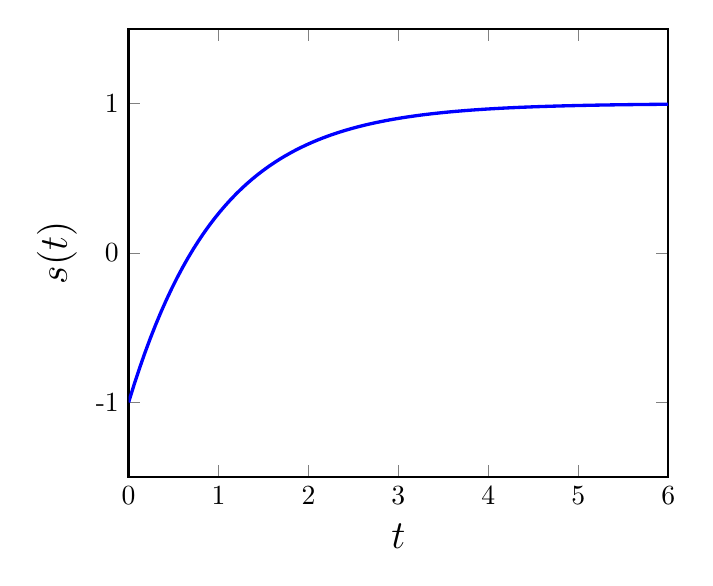
\begin{tikzpicture}%[baseline=0]
        \begin{axis}[
        scaled y ticks = false,
        axis line style = thick,
        %height=5cm,
        %width=9cm,
        %axis x line=center,
        %axis y line=center,
        xmin=0,
        xmax=6.0,
        ymin=-1.5,
        ymax=1.5,
        xlabel={$t$},
        ylabel={$s(t)$},
        %xlabel style={below right},
        %ylabel style={above left},
        yticklabels={-1,0,1},
        ytick={-1,0,1.0},
        y tick label style={anchor=east},
        label style={font=\Large},
        ]
        \addplot [very thick,color=blue,domain=0:6, samples=101]{1-2*exp(-x)};
        \end{axis}
    \end{tikzpicture}

    \caption{Représentation de la solution générale de l'équation différentielle~(\ref{eq-diff1}). On vérifie lors 
             du tracé que l'on observe bien les principales propriétes du signal (i.e conditions initiales, 
             valeurs finales).\label{fig-solution}}
\end{figure}

La solution générale de l'équation différentielle~(\ref{eq-diff1}) est donc donnée par, 
\begin{bequation}[ams align]
s(t)=1-2e^{-t}.
\end{bequation}
Nous laissons au lecteur le soin de vérifier que cette fonction est solution 
de l'équation~\ref{eq-diff1}, et qu'elle respecte notamment les conditions initiales. 
Le graphe de la solution est également présenté (\Cref{fig-solution}).

%%%%%%%%%%%%%%%%%%%%%%%%%%%%%%%%%%%%%%%%%%%%%%%%%%%%%%%%%%%%%%%%
\paragraph{Résolution par application de la transformée de Laplace}
%%%%%%%%%%%%%%%%%%%%%%%%%%%%%%%%%%%%%%%%%%%%%%%%%%%%%%%%%%%%%%%%

La transformée de Laplace est linéaire. Il nous est alors possible
de l'appliquer aux différents termes de l'équation différentielle~(\ref{eq-diff1}) séparemment.
On obtient pour chacuns des termes :
\begin{align*}
    \laplace{s(t)} &= S(p), \\
    \laplace{\devi{s(t)}{}} &= pS(p)-s(0) = pS(p) +1, \\
    \laplace{\devi{s(t)}{2}} &= p^2S(p)-ps(0)-s'(0) = p^2S(p) + p -2,\\
    \laplace{u(t)} &= \dfrac{1}{p}.
\end{align*}

L'équation différentielle~(\ref{eq-diff1}) devient dans le domaine de Laplace :
\begin{align*}
p^2S(p)+p-2+2pS(p)+2+S(p)=\dfrac{1}{p} 
\end{align*}

En réarrangeant cette expression, il est possible de déterminer la forme de la réponse 
$S(p)$ dans le domaine de Laplace.

\begin{align*}
    S(p)\left(p^2+2p+1\right)+p&=\dfrac{1}{p} \\
    S(p)\left(p+1\right)^2 &= \dfrac{1-p^2}{p}\\
    S(p)&= \dfrac{1-p^2}{p\left(p+1\right)^2}
\end{align*}

Cette forme \og n'existant\fg pas dans les tableaux de transformation de Laplace usuels, nous allons décomposer cette
fraction rationnelle en éléments simples (\Cref{annexe-DES}).

$$
S(p)=\dfrac{A}{p}+\dfrac{B}{p+1}+\dfrac{C}{(p+1)^2}
$$

Par identification, 
$$
S(p)=\dfrac{A(p+1)^2+Bp(p+1)+Cp}{p(p+1)^2}=\dfrac{1-p^2}{p\left(p+1\right)^2}
$$

$$
\begin{cases}
    A+B&=-1 \\
    2A+B+C&=0 \\
    A&=1   
\end{cases}\Rightarrow
\begin{cases}
    B&=-2\\
    C&=0
\end{cases}
$$

La réponse $S(p)$ se décompose donc de la façon suivante en éléments simples:
$$
S(p)=\dfrac{1}{p}-\dfrac{2}{p+1}
$$
Il est maintenant plus aisé d'appliquer la transformation de Laplace inverse, 
en utilisant le tableau des transformées de Laplace usuels (c.f lignes 3 et 7 du tableau de l'\Cref{annexe-lap}) 
pour obtenir la réponse temporelle $s(t)$. Notamment,
$$
\laplacei{\dfrac{1}{p}}=1
$$
et
$$
\laplacei{\dfrac{2}{p+1}}=2e^{-t}
$$
soit 
\begin{bequation}[ams align]
    \laplacei{S(p)}=s(t)=1-2e^{-t}
\end{bequation}

Comme attendu, les deux méthodes donnent le même résultat, cependant la transformée de Laplace permet de définir dans 
le domaine de Laplace, une relation direct entre l'entrée et la sortie d'un système. C'est la fonction de transfert 
qui réalise ce lien.

%%%%%%%%%%%%%%%%%%%%%%%%%%%%%%%%%%%%%%%%%%%%%%%%%%%%%%%%%%%%%%%%%%%%%%%%%%%%
\section{Fonction de Transfert}
%%%%%%%%%%%%%%%%%%%%%%%%%%%%%%%%%%%%%%%%%%%%%%%%%%%%%%%%%%%%%%%%%%%%%%%%%%%%

%%%%%%%%%%%%%%%%%%%%%%%%%%%%%%%%%%%%%%%%%%%%%%ù
\subsection{Définition}
%%%%%%%%%%%%%%%%%%%%%%%%%%%%%%%%%%%%%%%%%%%%%%ù

La fonction de transfert $H(p)$ d'un système est donnée par le rapport de la 
sortie $S(p)$ et l'entrée $E(p)$ dans le domaine de Laplace. 
\begin{bequation}[ams align]
H(p)=\dfrac{S(p)}{E(p)}
\end{bequation}
ou encore,
\begin{bequation}[ams align]
    S(p)=H(p)E(p)\label{eq-she}
\end{bequation}

Cette fonction $H(p)$, également appelé \textbf{transmittance}, caractérise le système de façon univoque.
Pour une entrée donnée il est possible de prévoir la sortie d'un système caractérisé par 
sa fonction de transfert $H(p)$

%%%%%%%%%%%%%%%%%%%%%%%%%%%%%%%%%%%%%%%%%%%%%%%%%%%%%%%%%%%%%%%%%%%%%%
\subsection{Fonction de transfert et réponse impulsionnelle}
%%%%%%%%%%%%%%%%%%%%%%%%%%%%%%%%%%%%%%%%%%%%%%%%%%%%%%%%%%%%%%%%%%%%%%
À partir de l'équation~\ref{eq-she}, le lien entre la fonction de transfert
et la réponse impulsionnelle paraît évident. Pour une impulsion de Dirac 
en entrée, la réponse impulsionnelle est alors simplement la fonction 
de transfert puisque $\laplace{\delta(t)}=E(p)=1$. Autrement dit, la fonction de 
transfert d'un système est la réponse impulsionnelle dans le domaine de Laplace.
Formellement, si $h(t)$ est la réponse impulsionnelle d'un système alors,
$$
H(p) = \laplace{h(t)}
$$
D'après la propriété du produit de convolution, nous savons que le produit de deux fonctions
dans le domaine de Laplace correspond au produit de convolution de ces deux fonctions
dans le domaine temporelle, dans le cas de l'équation~\ref{eq-she},
$$
s(t)=\laplacei{S(p)}=\laplacei{H(p)E(p)}=\int_{-\infty}^{+\infty}h(t-\tau)e(\tau)\dd{\tau}
$$
ou encore,
$$
s(t)=(h*e)(t)
$$
ce qui exprime que \textbf{la réponse d'un système est donnée par le produit de convolution de l'entrée  et la réponse impulsionnelle.}

%%%%%%%%%%%%%%%%%%%%%%%%%%%%%%%%%%%%%%%%%%%%%%%%%%%%%%%%%%%%%%%%%%%%%%%%%%%%
\subsection[Représentation de la fonction de transfert]{Représentations algébrique et graphique de la fonction de transfert}
%%%%%%%%%%%%%%%%%%%%%%%%%%%%%%%%%%%%%%%%%%%%%%%%%%%%%%%%%%%%%%%%%%%%%%%%%%%%

D'après la loi fréquentielle (\Cref{eq-lfreq}), la fonction de transfert 
d'un \gls{slci}~peut s'écrire sous la forme d'une fraction rationnelle,
\begin{bequation}[ams align]
H(p)=\dfrac{\sum\limits_{i=0}^{m}b_ip^i}{\sum\limits_{i=0}^{n}a_ip^i}. \label{eq-ftgen}
\end{bequation}

Il existe différentes façons équivalentes d'écrire cette fonction de transfert. 
Nous allons en introduire deux :
la forme canonique et la forme factorisée. La forme canonique permet de faire apparaître 
les intégrateurs purs du système. La forme factorisée utilise les racines de la 
fraction rationnelle définissant la fonction de transfert. 
Pour montrer l'équivalence de ces représentations nous allons les 
construire à partir de la forme générale de l'\cref{eq-ftgen} et ou de la connaissance des pôles et zéros de 
la fonction de transfert.

Une fonction de transfert peut être vue comme le fraction de deux polynômes (i.e fraction rationnelle):
un polynôme au numérateur $N(p)$ et un polynôme au dénominateur $D(p)$.
$$
H(p)=\dfrac{N(p)}{D(p)}
$$
Ces polynômes possèdent des racines dans $\mathbb{C}$. Les \textbf{racines de $N(p)$ sont 
dits les zéros de $H(p)$ }et les \textbf{racines de $D(p)$ 
sont dits les pôles de $H(p)$}. Il en vient qu'une fonction de transfert possède $m$ zéros et $n$ pôles.

%%%%%%%%%%%%%%%%%%%%%%%%%%%%%%%%%%%%%%%%%%%%%%ù
\paragraph{Exemple}
%%%%%%%%%%%%%%%%%%%%%%%%%%%%%%%%%%%%%%%%%%%%%%ù
Reprenons l'équation différentielle de la section précédente, dans les conditions de Heaviside, afin de construire 
la fonction de transfert qui lui est associée. 
\begin{align}                                                                                                                 
\devi{s(t)}{2}+2\devi{s(t)}{} + s(t) = e(t)  
\end{align}  
La transformée de Laplace de cette équation nous donne,
\begin{align*}                                        
	p^2S(p)+2pS(p)+S(p)&=E(p)\\
	S(p)\left(p^2+2p+1\right)&=E(p)\\
	S(p)&=\dfrac{1}{p^2+2p+1}E(p)
\end{align*}  
La fonction de transfert associée à cette équation différentielle est donc 
$$
H(p)=\dfrac{1}{p^2+2p+1}
$$
Il est aisé de constater que la fonction de transfert est d'ordre deux et ne possède pas de zéro.


%%%%%%%%%%%%%%%%%%%%%%%%%%%%%%%%%%%%%%%%%%%%%%ù
\paragraph{Forme canonique de la fonction de transfert}
%%%%%%%%%%%%%%%%%%%%%%%%%%%%%%%%%%%%%%%%%%%%%%ù
Développons les sommes de l'\cref{eq-ftgen},
$$
H(p)=\dfrac{b_0+b_1p+b_2p^2+\ldots+b_mp^m}{a_0+a_1p+a_2p^2+\ldots+a_np^n}.
$$
La forme canonique dépend du nombre d'intégrateur du système. 
Par exemple, si $a_0$ est non nul, l'expression précédente se factorise sous la forme,
$$
H(p)=K_0\cdot\dfrac{1+b'_1p+b'_2p^2+\ldots+b'_mp^m}{1+a'_1p+a'_2p^2+\ldots+a'_np^n}.
$$
avec $K_0=\dfrac{b_0}{a_0}$, $a'_i=\dfrac{a_i}{a_0}$ et $b'_i=\dfrac{b_i}{b_0}$. 
Dans ce cas, le système est dit de classe 0 et ne possède aucun intégrateur.

Si maintenant $a_0$ est nul et $a_1$ non nul, la fonction de transfert peut s'écrire,
$$
H(p)=\dfrac{K_1}{p}\cdot\dfrac{1+b'_1p+b'_2p^2+\ldots+b'_mp^m}{1+a'_1p+a'_2p^2+\ldots+a'_{n-1}p^{n-1}}.
$$
avec $K_1=\dfrac{b_0}{a_1}$, $a'_i=\dfrac{a_{i+1}}{a_1}$ et $b'_i=\dfrac{b_i}{b_0}$.
Dans ce cas, le système est dit de classe 1 et possède un intégrateur.

On généralise donc la forme canonique de la fonction de transfert d'un système de classe $\alpha$ sous la forme,
\begin{bequation}[ams align]
H(p)=\dfrac{K_\alpha}{p^\alpha}\cdot\dfrac{\sum\limits_{i=0}^{m}b'_i p^i}{\sum\limits_{i=0}^{n-\alpha}a'_ip^i} \label{eq-ftcan} 
\end{bequation}
où $K_\alpha=\dfrac{b_0}{a_\alpha}$ est \textbf{le gain statique}, $\alpha$ est \textbf{la classe du système} 
et les coefficients de la forme canonique $a'_i$ et $b'_i$ sont déterminés à partir des coefficients 
de l'équation différentielle régissant le système\footnote{Pour simplifier la notation, 
les primes des coefficients de la forme canonique peuvent être omis, cependant 
ceux-ci restent toujours différents des coefficients de l'équation différentielle.}.

En posant respectivement $N(p)$ et $D(p)$ les polynômes du numérateur et du dénomintateur.
La forme canonique de la fonction de transfert s'écrira également très souvent:
$$
H(p)=\dfrac{K_\alpha N(p)}{p^\alpha D(p)}
$$
On rappellera que sous cette forme les polynômes $N(p)$ et $D(p)$ sont de la forme 
$$
1+a_1p+a_2p^2+\ldots+a_{n-\alpha}p^{n-\alpha}
$$
et donc $N(0)=1$ et $D(0)=1$.


%%%%%%%%%%%%%%%%%%%%%%%%%%%%%%%%%%%%%%%%%%%%%%ù
\paragraph{Exemple de forme canonique}
%%%%%%%%%%%%%%%%%%%%%%%%%%%%%%%%%%%%%%%%%%%%%%ù
Soit un système décrit par la fonction de transfert suivante:
$$
H(p)=\dfrac{2p+5}{p^3+2p^2+4p}
$$
Le coefficient d'ordre 0 étant nul au dénominateur, le système est de classe 1, 
la forme canonique de cette fonction de transfert est 
donc\footnote{Il est d'usage en automatique d'écrire les nombres rationnels 
par leurs valeurs numériques plutôt que par leurs fractions. } donnée par
\begin{align*}
H(p)=\dfrac{K(0.4p+1)}{p(0.25p^2+0.5p+1)},
\end{align*}
où le gain statique $K=$1.25.

%%%%%%%%%%%%%%%%%%%%%%%%%%%%%%%%%%%%%%%%%%%%%%ù
\paragraph{Forme factorisée de la fonction de transfert}
%%%%%%%%%%%%%%%%%%%%%%%%%%%%%%%%%%%%%%%%%%%%%%ù
Soient les pôles $p_i$ avec $i\in[1,n]$ et les zéros $z_j$ 
avec $j\in[1,m]$ de la fonction de transfert $H(p)$. 
Il est alors possible de factoriser par les pôles et les zéros pour écrire la fonction de 
transfert sous la forme:
\begin{bequation}[ams align]
H(p)=k\cdot\dfrac{\prod\limits_{j=0}^{m}(p-z_j)}{\prod\limits_{i=0}^{n}(p-p_i)},
\end{bequation}
avec $k=\dfrac{b_m}{a_n}$. On remarquera que cette constante $k$ 
n'est pas le gain statique de la forme canonique.

Cette forme factorisée est très utile pour la représentation graphique
de la réponse harmonique (c.f~\cref{chap-anafreq}).

%%%%%%%%%%%%%%%%%%%%%%%%%%%%%%%%%%%%%%%%%%%%%%ù
\paragraph{Exemple de fonction de transfert factorisée}
%%%%%%%%%%%%%%%%%%%%%%%%%%%%%%%%%%%%%%%%%%%%%%ù

Soit la fonction de transfert $H(p)$ tel que
$$
H(p)=\dfrac{6p+12}{2p^2+4p+1.5}	
$$
En factorisant par les coefficients d'ordre maximum au numérateur et au dénominateur, et en observant 
que la fonction de transfert possède un zéro ($z_1=-2$) et deux pôles ($p_1=-1.5$ et $p_2=-0.5$), 
on peut réécrire $H(p)$ sous sa forme factorisée:
$$
H(p)=\dfrac{6}{2}\cdot\dfrac{p+2}{p^2+2p+0.75}
$$
La fonction de transfert possède un zéro ($z_1=-2$) et deux pôles ($p_1=-1.5$ et $p_2=-0.5$).
Elle peut alors s'écrire :
$$
H(p)=\dfrac{k(p+2)}{(p+1.5)(p+0.5)}
$$
avec $k=3$.
	
%%%%%%%%%%%%%%%%%%%%%%%%%%%%%%%%%%%%%%%%%%%%%%ù
\paragraph{Carte des pôles et zéros d'une fonction de transfert}
%%%%%%%%%%%%%%%%%%%%%%%%%%%%%%%%%%%%%%%%%%%%%%ù

Il est également possible de représenter une fonction de transfert graphiquement à 
l'aide d'une carte des pôles et des zéros dans le plan complexe (les racines d'un polynôme 
pouvant être complexes). Dans ce type de représentation, les pôles 
sont représentés par des ($\times$) et les zéros par des ($\circ$).
La carte des pôles et des zéros d'une fonction de transfert est essentielle 
pour la construction du lieu d'Evans\footnote{Walter Richard Evans, (1920-1999), 
ingénieur, automaticien américain} pour l'étude des systèmes asservis.

%%%%%%%%%%%%%%%%%%%%%%%%%%%%%%%%%%%%%%%%%%%%%%ù
\paragraph{Exemple de carte de pôles et zéros d'une fonction de transfert}
%%%%%%%%%%%%%%%%%%%%%%%%%%%%%%%%%%%%%%%%%%%%%%ù

Soit $H(p)$ une fonction de transfert telle que,
\begin{align}
H(p)=\dfrac{p-1}{p^2+2p+2}\label{eq-ft_carte}
\end{align}
Cette fonction de transfert possède un zéro réel ($z_1=1$) et deux 
pôles complexes conjugués ($p_{1,2}=-1\pm j$).
La forme factorisée de $H(p)$ est donc
\begin{align} 
    H(p)=\dfrac{p-1}{(p+1+j)(p+1-j)}
\end{align}

La~\cref{fig-carte} présente la carte des pôles de cette fonction de transfert.
\begin{figure}[!h]
    \begin{center}
    \tikzsetnextfilename{carte-chap0_ext}
    \begin{tikzpicture}
    \begin{axis}
    [   scaled y ticks = false,
        axis line style = thick,
        axis x line=center,
        axis y line=center,
        xmin=-2.5,
        xmax=2.5,
        ymin=-1.5,
        ymax=1.5,
        xlabel={$\boldsymbol{\Re{p}}$},
        ylabel={$\boldsymbol{\Im{p}}$},
        xlabel style={below right},
        ylabel style={above left},
        yticklabels={-1,0,1},
        ytick={-1,0,1.0},
        y tick label style={anchor=east}
    ]
    \addplot[mark=x,utb,only marks,mark size=5pt] coordinates{(-1,1) (-1,-1)};
    \addplot[mark=o,utr,mark size=5pt] coordinates{ (1,0) };
    \end{axis}
\end{tikzpicture}

\end{center}
\caption{Exemple d'une carte de pôles et zéros associés 
    à la fonction de transfert~\Cref{eq-ft_carte}\label{fig-carte} }
\end{figure}





%%%%%%%%%%%%%%%%%%%%%%%%%%%%%%%%%%%%%%%%%%%%%%%%%%%%%%%%%%%%%%%%%%%%%%
%%%%%%%%%%%%%%%%%%%%%%%%%%%%%%%%%%%%%%%%%%%%%%%%%%%%%%%%%%%%%%%%%%%%%%
%%%%%%%%%%%%%%%%%%%%%%%%%%%%%%%%%%%%%%%%%%%%%%%%%%%%%%%%%%%%%%%%%%%%%%
%\section{Exercices du chapitre}
%%%%%%%%%%%%%%%%%%%%%%%%%%%%%%%%%%%%%%%%%%%%%%%%%%%%%%%%%%%%%%%%%%%%%%
%%%%%%%%%%%%%%%%%%%%%%%%%%%%%%%%%%%%%%%%%%%%%%%%%%%%%%%%%%%%%%%%%%%%%%
%%%%%%%%%%%%%%%%%%%%%%%%%%%%%%%%%%%%%%%%%%%%%%%%%%%%%%%%%%%%%%%%%%%%%%
%\small
%%%%%%%%%%%%%%%%%%%%%%%%%%%%%%%%%%%%%%%%%%%%%%%%%%%%%%%%%%%%%%%%%%%%%%%%%%%%%%%%%
\exercice{Décomposition en signaux usuels}
%%%%%%%%%%%%%%%%%%%%%%%%%%%%%%%%%%%%%%%%%%%%%%%%%%%%%%%%%%%%%%%%%%%%%%%%%%%%%%%%

Soit la fonction porte $p_a(t)$ définie graphiquement de la façon suivante :

\tikzsetnextfilename{exercice_2-chap0-ext}
\begin{center}
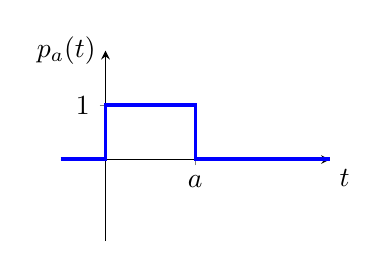
\begin{tikzpicture}[baseline=0]
   \begin{axis}[
        height=4cm,
        width=5cm,
        axis x line=center,
        axis y line=center,
        xmin=-1,
        xmax=5,
        ymin=-1.5,
        ymax=2.0,
        xlabel={$t$},
        ylabel={$p_a(t)$},
        xlabel style={below right},
        ylabel style={left},
        yticklabels={1},
        ytick={1},
        y tick label style={anchor=east},
        xticklabels={$a$},
        xtick={2},
        x tick label style={anchor=north},
        ]
        \addplot [very thick,color=blue,const plot] coordinates 
        {(-1,0.01) (0,0.01) (0,1) (2,1)  (2,0.01) (5,0.01) };
        \end{axis}
\end{tikzpicture}
\end{center}

\question{}
\textbf{Déterminer $p_a(t)$ (la fonction porte) à l'aide de fonctions échelons. 
et donner sa transformée de Laplace.}
\newline

Soit la fonction $u_a(t)$ définie graphiquement de la façon suivante :

\tikzsetnextfilename{exercice_3-chap0-ext}
\begin{center}
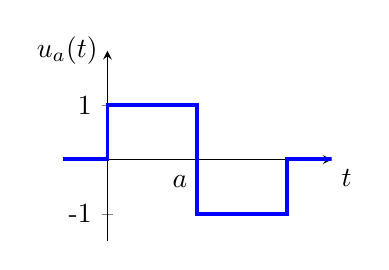
\begin{tikzpicture}[baseline=0]
   \begin{axis}[
   height=4cm,
   width=5cm,
      axis x line=center,
        axis y line=center,
        xmin=-1,
        xmax=5,
        ymin=-1.5,
        ymax=2.0,
        xlabel={$t$},
        ylabel={$u_a(t)$},
        xlabel style={below right},
        ylabel style={left},
        yticklabels={-1,1},
        ytick={-1,1},
        y tick label style={anchor=east},
        xticklabels={$a$},
        xtick={2},
        x tick label style={below left},
        ]
        \addplot [very thick,color=blue,const plot] coordinates 
        {(-1,0.01) (0,0.01) (0,1) (2,1)  (2,-1) (4,-1) (4,0.01) (5,0.01)  };
        \end{axis}
\end{tikzpicture}
\end{center}

\question{}
\textbf{Déterminer $u_a(t)$ en fonction de $p_a(t)$ et donner sa 
transformée de Laplace.}
\newline

Soit la fonction $g_0(t)$ définie graphiquement de la façon suivante :

\tikzsetnextfilename{exercice_4-chap0-ext}
\begin{center}
\begin{tikzpicture}[baseline=0]
   \begin{axis}[
   height=4cm,
   width=5cm,
      axis x line=center,
        axis y line=center,
        xmin=-1,
        xmax=5,
        ymin=-1.5,
        ymax=2.0,
        xlabel={$t$},
        ylabel={$g_0(t)$},
        xlabel style={below right},
        ylabel style={left},
        yticklabels={$E$},
        ytick={1},
        y tick label style={left},
        xticklabels={$\dfrac{T}{2}$,$T$},
        xtick={2,4},
        x tick label style={below},
        ]
        \addplot [very thick,color=blue,domain=-1:0, samples=101]{0.05};
        \addplot [very thick,color=blue,domain=0:2, samples=101]{0.5*x};
        \addplot [very thick,color=blue,domain=2:4, samples=101]{-0.5*x+2};
        \addplot [very thick,color=blue,domain=4:5, samples=101]{0.05};
        \end{axis}
\end{tikzpicture}
\end{center}

\question{}
\textbf{Déterminer $g_0(t)$ en fonction de $u_a(t)$ et donner sa 
transformée de Laplace.}

\newpage
%%%%%%%%%%%%%%%%%%%%%%%%%%%%%%%%%%%%%%%%%%%%%%%%%%%%%%%%%%%%%%%%%%%%%%%%%%%%%%%%
\exercice{Décomposition en signaux usuels (2)}
%%%%%%%%%%%%%%%%%%%%%%%%%%%%%%%%%%%%%%%%%%%%%%%%%%%%%%%%%%%%%%%%%%%%%%%%%%%%%%%%

\question{}
\textbf{Déterminer la transformée de Laplace des signaux suivants en 
décomposant le signal en somme d'échelons et de rampes; $g(t)$ étant un signal
périodique.}

\tikzsetnextfilename{exercice_4-1-chap0-ext}
\begin{center}
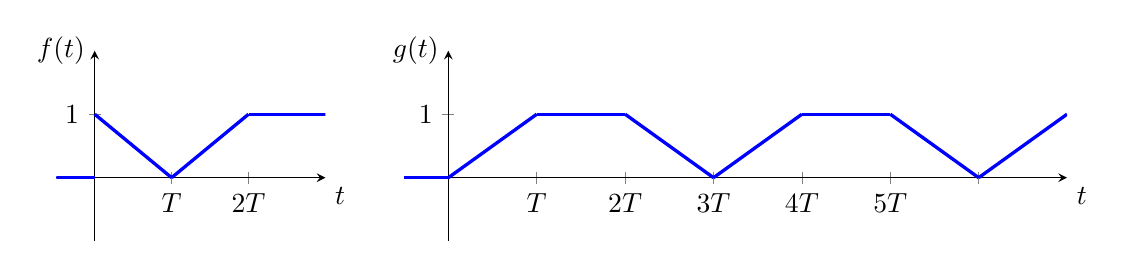
\begin{tikzpicture}[baseline=0]
   \begin{axis}[
        name=first,   
        height=4cm,
        width=5cm,
        axis x line=center,
        axis y line=center,
        xmin=-1,
        xmax=6,
        ymin=-1,
        ymax=2.0,
        xlabel={$t$},
        ylabel={$f(t)$},
        xlabel style={below right},
        ylabel style={left},
        yticklabels={1},
        ytick={1},
        y tick label style={left},
        xticklabels={0,$T$,$2T$},
        xtick={0,2,4},
        x tick label style={below},
        ]
        \addplot [very thick,color=blue,domain=-1:0, samples=101]{0};
        \addplot [very thick,color=blue,domain=0:2, samples=101]{-0.5*x+1};
        \addplot [very thick,color=blue,domain=2:4, samples=101]{0.5*x-1};
        \addplot [very thick,color=blue,domain=4:6, samples=101]{1};
        \end{axis}
   \begin{axis}[
        at=(first.east),anchor=west,xshift=1cm,
        height=4cm,
        width=10cm,
        axis x line=center,
        axis y line=center,
        xmin=-1,
        xmax=14,
        ymin=-1,
        ymax=2.0,
        xlabel={$t$},
        ylabel={$g(t)$},
        xlabel style={below right},
        ylabel style={left},
        yticklabels={1},
        ytick={1},
        y tick label style={left},
        xticklabels={0,$T$,$2T$,$3T$,$4T$,$5T$},
        xtick={0,2,4,6,8,10,12},
        x tick label style={below},
       ]
        \addplot [very thick,color=blue,domain=-1:0, samples=101]{0};
        \addplot [very thick,color=blue,domain=0:2, samples=101]{0.5*x};
        \addplot [very thick,color=blue,domain=2:4, samples=101]{1};
        \addplot [very thick,color=blue,domain=4:6, samples=101]{-0.5*x+3};
        \addplot [very thick,color=blue,domain=6:8, samples=101]{0.5*x-3};
        \addplot [very thick,color=blue,domain=8:10, samples=101]{1};
        \addplot [very thick,color=blue,domain=10:12, samples=101]{-0.5*x+6};
        \addplot [very thick,color=blue,domain=12:14, samples=101]{0.5*x-6};
   \end{axis}
\end{tikzpicture}
\end{center}

%%%%%%%%%%%%%%%%%%%%%%%%%%%%%%%%%%%%%%%%%%%%%%%%%%%%%%%%%%%%%%%%%%%%%%%%%%%%%%%%
\exercice{\'Etude d'équations différentielles}
%%%%%%%%%%%%%%%%%%%%%%%%%%%%%%%%%%%%%%%%%%%%%%%%%%%%%%%%%%%%%%%%%%%%%%%%%%%%%%%%

Un système linéaire est décrit par les équations différentielles suivantes :
$$
\devi{s(t)}{2} + 110 \devi{s(t)}{} + 1000 s(t) = \devi{x(t)}{} + 30 x(t)
$$
et 
$$
\devi{x(t)}{} + x(t) = K e(t) 
$$

$e(t)$ est l'entrée du système, la sortie $s(t)$ et $x(t)$ est une variable
interne. On se place dans les conditions d'Heaviside (c.a.d conditions 
initiales nulles).\newline

\question{}
\textbf{\'Ecrire ces équations dans le domaine de Laplace (avec 
$p\in\mathbb{C}$ la variable complexe).}

\question{}
\textbf{Tracer le schéma fonctionnel complet du système.}

\question{}
\textbf{Déterminer la fonction de transfert du système.}
\newline

On sollicite le système avec un échelon $e(t)=E_0 u(t)$

\question{}
\textbf{Déterminer la valeur finale de la sortie et la tangente à l'origine.}

\question{}
\textbf{Déterminer la sortie $s(t)$ et tracer le signal.}

\exercice{Fonction de transfert, réponse temporelle}

\question{}
\textbf{Pour chacunes des équations différentielles suivantes, 
déterminer la fonction de transfert $H(p) = S(p)/E(p)$, les valeurs initiales
et finales ainsi que leurs réponses temporelles $s(t)$.}

\begin{itemize}
\item[\textbf{(1)}] $\devi{s(t)}{} + 2s(t) = e(t) $ avec $s(0)=2$ 
                    et $e(t) = e^{-t}$
\item[\textbf{(2)}] $\devi{s(t)}{2} + 3 \devi{s(t)}{} + 2s(t) 
                    = \devi{e(t)}{} + e(t)$ 
                    avec $\devi{s(0)}{}=s(0)=0$ et $e(t) = e^{-3t}$
\item[\textbf{(3)}] $\devi{s(t)}{2} + 2\devi{s(t)}{} + s(t)  = e(t)$ 
                    avec $\devi{s(0)}{}=s(0)=0$ et $e(t) = e^{-2t}$
\item[\textbf{(4)}] $\devi{s(t)}{2} + \devi{s(t)}{} + s(t) = e(t)$ 
                    avec $\devi{s(0)}{}=s(0)=0$ et $e(t) = 1$
\end{itemize}

%%%%%%%%%%%%%%%%%%%%%%%%%%%%%%%%%%%%%%%%%%%%%%%%%%%%%%%%%%%%%%%%%%%%%%%%%%%%%%%%
\exercice{Transformée de Laplace d'une fonction périodique}
%%%%%%%%%%%%%%%%%%%%%%%%%%%%%%%%%%%%%%%%%%%%%%%%%%%%%%%%%%%%%%%%%%%%%%%%%%%%%%%%

Nous rappelons que dans le cas générale, 
la transformée de Laplace d'une fonction causale et périodique $f(t)$ de 
période $T$ est donné par :
$$
F(p) = \dfrac{F_0(p)}{1-e^{-Tp}}
$$
où $F_0(p)$ est la transformée de Laplace du motif $f_0(t)$ égal à $f(t)$ 
sur le segment $[0,T]$ et nulle partout ailleurs.

\question{}
\textbf{Déterminer la transformée de Laplace $F(p)$ de la fonction 
        temporelle $f(t)$ causale et périodique, définie par la figure 
        ci-dessous :}

\begin{center}
    \tikzsetnextfilename{exercice_1-chap0-ext}
    \begin{tikzpicture}
        \begin{axis}[
        height=5cm,
        width=0.75\textwidth,  
        axis x line=center,
        axis y line=center,
        xmin=-1,
        xmax=16,
        ymin=-1.5,
        ymax=1.5,
        xlabel={$t$},
        ylabel={$f(t)$},
        xlabel style={below right},
        ylabel style={above left},
        yticklabels={$-E$,$E$},
        ytick={-1,1},
        y tick label style={anchor=east},
        xticklabels={$\dfrac{T}{2}$,$T$,$2T$},
        xtick={2,4,8},
        x tick label style={below},
        extra x ticks={6},
        extra x tick labels={$\dfrac{3T}{2}$},
        extra x tick style={
        xticklabel style={above},}
        ]
        \addplot [very thick,color=blue,domain=0:2  ,samples=101]
        {0.5*x};
        \addplot [very thick,color=blue,domain=2:6  ,samples=101]
        {-0.5*x+2};
        \addplot [very thick,color=blue,domain=6:10 ,samples=101]
        {0.5*x-4};
        \addplot [very thick,color=blue,domain=10:14,samples=101]
        {-0.5*x+6};
        \end{axis}
    \end{tikzpicture}
\end{center}

Pour répondre à la question on pourra s'aider des résultats de 
l'exercice~\ref{exe-1_chap0} pour progressivement construire le motif de 
base de cette fonction périodique à savoir $f_0(t)=f(t)$ pour 
$0\leq t\leq2T$ en fonction de $g_0(t)$.

%%%%%%%%%%%%%%%%%%%%%%%%%%%%%%%%%%%%%%%%%%%%%%%%%%%%%%%%%%%%%%%%%%%%%%%%%%%%%%%%
\exercice{Cartes des pôles et zéros}
%%%%%%%%%%%%%%%%%%%%%%%%%%%%%%%%%%%%%%%%%%%%%%%%%%%%%%%%%%%%%%%%%%%%%%%%%%%%%%%%

\question{}
Tracer la carte des pôles et zéros des fonctions de transferts suivantes:
\begin{itemize}
    \item[(a)] $H_1(p)=\dfrac{4p}{p^3+2p^2+8p+16}$
    \item[(b)] $H_2(p)=\dfrac{(p+1)}{(p^2+2p+2)(p+4)}$
    \item[(c)] $H_3(p)=\dfrac{(p+1)}{(p^2+2p+1)(p^2+p+0.5)}$
\end{itemize}
%%%%%%%%%%%%%%%%%%%%%%%%%%%%%%%%%%%%%%%%%%%%%%%%%%%%%%%%%%%%%%%%%%%%%%%%%%%%%%%%
%%%%%%%%%%%%%%%%%%%%%%%%%%%%%%%%%%%%%%%%%%%%%%%%%%%%%%%%%%%%%%%%%%%%%%%%%%%%%%%%
%%%%%%%%%%%%%%%%%%%%%%%%%%%%%%%%%%%%%%%%%%%%%%%%%%%%%%%%%%%%%%%%%%%%%%%%%%%%%%%%
%%%%%%%%%%%%%%%%%%%%%%%%%%%%%%%%%%%%%%%%%%%%%%%%%%%%%%%%%%%%%%%%%%%%%%%%%%%%%%%%
%exercice_chap0.tex


%\setcounter{numexos}{0}
%\normalsize
%\newpage
%%%%%%%%%%%%%%%%%%%%%%%%%%%%%%%%%%%%%%%%%%%%%%%%%%%%%%%%%%%%%%%%%%%%%%
%%%%%%%%%%%%%%%%%%%%%%%%%%%%%%%%%%%%%%%%%%%%%%%%%%%%%%%%%%%%%%%%%%%%%%
%%%%%%%%%%%%%%%%%%%%%%%%%%%%%%%%%%%%%%%%%%%%%%%%%%%%%%%%%%%%%%%%%%%%%%
%\section{Corrigé des exercices}
%%%%%%%%%%%%%%%%%%%%%%%%%%%%%%%%%%%%%%%%%%%%%%%%%%%%%%%%%%%%%%%%%%%%%%
%%%%%%%%%%%%%%%%%%%%%%%%%%%%%%%%%%%%%%%%%%%%%%%%%%%%%%%%%%%%%%%%%%%%%%
%%%%%%%%%%%%%%%%%%%%%%%%%%%%%%%%%%%%%%%%%%%%%%%%%%%%%%%%%%%%%%%%%%%%%%
%\small
%%%%%%%%%%%%%%%%%%%%%%%%%%%%%%%%%%%%%%%%%%%%%%%%%%%%%%%%%%%%%%%%%%%%%%%%%%%%%%%%%
%%%%%%%%%%%%%%%%%%%%%%%%%%%%%%%%%%%%%%%%%%%%%%%%%%%%%%%%%%%%%%%%%%%%%%%%%%%%%%%%
\exercice{Décomposition en signaux usuels}
%%%%%%%%%%%%%%%%%%%%%%%%%%%%%%%%%%%%%%%%%%%%%%%%%%%%%%%%%%%%%%%%%%%%%%%%%%%%%%%%
%%%%%%%%%%%%%%%%%%%%%%%%%%%%%%%%%%%%%%%%%%%%%%%%%%%%%%%%%%%%%%%%%%%%%%%%%%%%%%%%

%%%%%%%%%%%%%%%%%%%%%%%%%%%%%%%%%%%%%%%%%%%%%%%%%%%%%%%%%%%%%%%%%%%%%%%%%%%%%%%%
\question{}
%%%%%%%%%%%%%%%%%%%%%%%%%%%%%%%%%%%%%%%%%%%%%%%%%%%%%%%%%%%%%%%%%%%%%%%%%%%%%%%%
\tikzsetnextfilename{ex1_1_corrige-chap0-ext}
\begin{center}
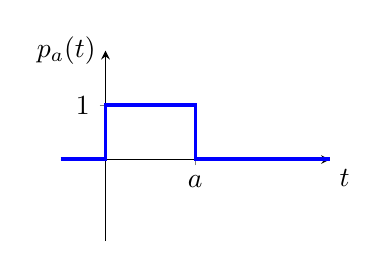
\begin{tikzpicture}
   \begin{axis}[
   height=4cm,
   width=5cm,
      axis x line=center,
        axis y line=center,
        xmin=-1,
        xmax=5,
        ymin=-1.5,
        ymax=2.0,
        xlabel={$t$},
        ylabel={$p_a(t)$},
        xlabel style={below right},
        ylabel style={left},
        yticklabels={1},
        ytick={1},
        y tick label style={anchor=east},
        xticklabels={$a$},
        xtick={2},
        x tick label style={anchor=north},
        ]
        \addplot [very thick,color=blue,const plot]  
        coordinates { (-1,0.01) (0,0.01) (0,1) (2,1)  (2,0.01) (5,0.01) };
        \end{axis}
\end{tikzpicture}
\tikzsetnextfilename{ex1_2_corrige-chap0-ext}
\begin{tikzpicture}
   \begin{axis}[
   height=4cm,
   width=5cm,
      axis x line=center,
        axis y line=center,
        xmin=-1,
        xmax=5,
        ymin=-1.5,
        ymax=2.0,
        xlabel={$t$},
        ylabel={$p_a(t)$},
        xlabel style={below right},
        ylabel style={left},
        yticklabels={1},
        ytick={1},
        y tick label style={anchor=east},
        xticklabels={$a$},
        xtick={2},
        x tick label style={below left},
        ]
        \addplot [very thick,color=col4,const plot]   
        coordinates { (-1, 0.01) (0, 0.01) (0 ,1)  (5,1) };
        \addplot [very thick,color=col3,const plot] 
        coordinates { (-1,-0.01) (0,-0.01) (2,-1) (5,-1) };
        \end{axis}
\end{tikzpicture}
\end{center}
$$
\color{blue}p_a(t)=\color{col4}u(t)\color{col3}-u(t-a)
$$ 
où $u(t)$ est la fonction échelon unité.

On rappel la transformée de Laplace d'une fonction retardée :
$$
\laplace{f(t-\tau)} = e^{-\tau p}F(p)
$$
La transformée de Laplace de $p_a(t)$ est donnée par : 
$$
P_a(p) = \laplace{p_a(t)}=\laplace{u(t)}-\laplace{u(t-a)}
=\dfrac{1}{p}(1-e^{-a p})
$$

%%%%%%%%%%%%%%%%%%%%%%%%%%%%%%%%%%%%%%%%%%%%%%%%%%%%%%%%%%%%%%%%%%%%%%%%%%%%%%%%
\question{}
%%%%%%%%%%%%%%%%%%%%%%%%%%%%%%%%%%%%%%%%%%%%%%%%%%%%%%%%%%%%%%%%%%%%%%%%%%%%%%%%

\tikzsetnextfilename{ex1_3_corrige-chap0-ext}
\begin{center}
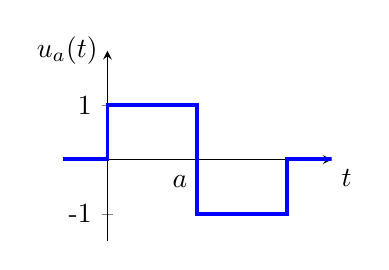
\begin{tikzpicture}
   \begin{axis}[
   height=4cm,
   width=5cm,
      axis x line=center,
        axis y line=center,
        xmin=-1,
        xmax=5,
        ymin=-1.5,
        ymax=2.0,
        xlabel={$t$},
        ylabel={$u_a(t)$},
        xlabel style={below right},
        ylabel style={left},
        yticklabels={-1,1},
        ytick={-1,1},
        y tick label style={anchor=east},
        xticklabels={$a$},
        xtick={2},
        x tick label style={below left},
        ]
        \addplot [very thick,color=blue,const plot] coordinates 
        {(-1,0.01) (0,0.01) (0,1) (2,1)  (2,-1) (4,-1) (4,0.01) (5,0.01)};
        \end{axis}
\end{tikzpicture}
\tikzsetnextfilename{ex1_4_corrige-chap0-ext}
\begin{tikzpicture}
   \begin{axis}[
    height=4cm,
    width=5cm,
    axis x line=center,
    axis y line=center,
    xmin=-1,
    xmax=5,
    ymin=-1.5,
    ymax=2.0,
    xlabel={$t$},
    ylabel={$u_a(t)$},
    xlabel style={below right},
    ylabel style={left},
    yticklabels={-1,1},
    ytick={-1,1},
    y tick label style={anchor=east},
    xticklabels={$a$},
    xtick={2},
    x tick label style={below left},
    ]
    \addplot[very thick,color=col4,const plot]    
    coordinates { (-1, 0.01) (0, 0.01) (0,1)  (2 ,1) (2, 0.01) (5,0.01) };
    \addplot[very thick,color=col3,const plot]  
    coordinates { (-1,-0.01) (2,-0.01) (2,-1) (4,-1) (4,-0.01) };
    \end{axis}
\end{tikzpicture}
\end{center}
$$
\color{blue}u_a(t)=\color{col4}p_a(t)\color{col3}-p_a(t-a)
$$ 
où $p_a(t)$ est la fonction fonction porte construite précédemment.

La transformée de Laplace de $u_a(t)$ est donnée par :
$$
U_a(p)=\laplace{u_a(t)}=\laplace{p_a(t)}-\laplace{p_a(t-a)}
      =P_a(p)(1-e^{-a p})=\dfrac{(1-e^{-ap})^2}{p}
$$

%%%%%%%%%%%%%%%%%%%%%%%%%%%%%%%%%%%%%%%%%%%%%%%%%%%%%%%%%%%%%%%%%%%%%%%%%%%%%%%%
\question{}
%%%%%%%%%%%%%%%%%%%%%%%%%%%%%%%%%%%%%%%%%%%%%%%%%%%%%%%%%%%%%%%%%%%%%%%%%%%%%%%%

\tikzsetnextfilename{ex1_5_corrige-chap0-ext}
\begin{center}
\begin{tikzpicture}
    \begin{axis}[
    height=4cm,
    width=5cm,
    axis x line=center,
    axis y line=center,
    xmin=-1,
    xmax=5,
    ymin=-1.5,
    ymax=2.0,
    xlabel={$t$},
    ylabel={$g_0(t)$},
    xlabel style={below right},
    ylabel style={above left},
    yticklabels={$E$},
    ytick={1},
    y tick label style={left},
    xticklabels={$\dfrac{T}{2}$,$T$},
    xtick={2,4},
    x tick label style={below},
    ]
    \addplot[very thick,color=blue,domain=-1:0, samples=101]{0.05};
    \addplot[very thick,color=blue,domain=0:2, samples=101]{0.5*x};
    \addplot [very thick,color=blue,domain=2:4, samples=101]{-0.5*x+2};
    \addplot [very thick,color=blue,domain=4:5, samples=101]{0.05};
    \end{axis}
\end{tikzpicture}
\tikzsetnextfilename{ex1_6_corrige-chap0-ext}
\begin{tikzpicture}
    \begin{axis}[
    height=4cm,
    width=5cm,
    axis x line=center,
    axis y line=center,
    xmin=-1,
    xmax=5,
    ymin=-1.5,
    ymax=2.0,
    xlabel={$t$},
    ylabel={$\frac{\mathrm{d}g_0(t)}{\mathrm{d}t}$},
    xlabel style={below right},
    ylabel style={above left},
    yticklabels={$\dfrac{2E}{T}$},
    ytick={1},
    y tick label style={left},
    xticklabels={$\dfrac{T}{2}$,$T$},
    xtick={2,4},
    x tick label style={below},
    ]
    \addplot [very thick,color=blue,domain=-1:0, samples=101]{0.01};
    \addplot [very thick,color=blue,domain=0:2, samples=101]{1.0};
    \addplot [very thick,color=blue,domain=2:4, samples=101]{-1.0};
    \addplot [very thick,color=blue,domain=4:5, samples=101]{0.01};
    \end{axis}
\end{tikzpicture}
\end{center}
$$
g_0(t)=\dfrac{2E}{T}\int_{0}^{t}u_{T/2}(t)\,\,\mathrm{d}\tau
$$

On rappel la transformée de Laplace de l'intégrale d'une fonction:
$$
\laplace{\int_{0}^{t}f(t)\,\,\mathrm{d}\tau}=\dfrac{F(p)}{p}
$$


La transformée de Laplace de $g_0(t)$ est donnée par :
$$
G_0(p) = \laplace{g_0(t)}=\dfrac{2E}{T}\dfrac{(1-e^{-Tp/2})^2}{p^2}
$$

%%%%%%%%%%%%%%%%%%%%%%%%%%%%%%%%%%%%%%%%%%%%%%%%%%%%%%%%%%%%%%%%%%%%%%%%%%%%%%%%
%%%%%%%%%%%%%%%%%%%%%%%%%%%%%%%%%%%%%%%%%%%%%%%%%%%%%%%%%%%%%%%%%%%%%%%%%%%%%%%%
\exercice{Décomposition en signaux usuels (2)}
%%%%%%%%%%%%%%%%%%%%%%%%%%%%%%%%%%%%%%%%%%%%%%%%%%%%%%%%%%%%%%%%%%%%%%%%%%%%%%%%
%%%%%%%%%%%%%%%%%%%%%%%%%%%%%%%%%%%%%%%%%%%%%%%%%%%%%%%%%%%%%%%%%%%%%%%%%%%%%%%%

%%%%%%%%%%%%%%%%%%%%%%%%%%%%%%%%%%%%%%%%%%%%%%%%%%%%%%%%%%%%%%%%%%%%%%%%%%%%%%%%
%%%%%%%%%%%%%%%%%%%%%%%%%%%%%%%%%%%%%%%%%%%%%%%%%%%%%%%%%%%%%%%%%%%%%%%%%%%%%%%%
\exercice{\'Etude d'équations différentielles}
%%%%%%%%%%%%%%%%%%%%%%%%%%%%%%%%%%%%%%%%%%%%%%%%%%%%%%%%%%%%%%%%%%%%%%%%%%%%%%%%
%%%%%%%%%%%%%%%%%%%%%%%%%%%%%%%%%%%%%%%%%%%%%%%%%%%%%%%%%%%%%%%%%%%%%%%%%%%%%%%%

%%%%%%%%%%%%%%%%%%%%%%%%%%%%%%%%%%%%%%%%%%%%%%%%%%%%%%%%%%%%%%%%%%%%%%%%%%%%%%%%
\question{}
%%%%%%%%%%%%%%%%%%%%%%%%%%%%%%%%%%%%%%%%%%%%%%%%%%%%%%%%%%%%%%%%%%%%%%%%%%%%%%%%
La première équation différentielle dans le domaine de Laplace, donne : 
\begin{align*}
p^2S(p)+110pS(p)+1000S(p)=pX(p)+30X(p) \\
S(p) ( p^2+110p+1000) = (p+30)X(p) \\
S(p) = \dfrac{(p+30)}{(p^2+110p+1000)} X(p) 
\end{align*}
cette dernière expression est de la forme :
\begin{align}
S(p) = H_2(p) X(p)
\label{eq-h2}
\end{align}
où $H_2(p)$ est une fonction de transfert d'un SLCI d'entrée $X(p)$ 
et de sortie $S(p)$.
\begin{center}
\tikzsetnextfilename{ex_2_corrige-chap0-ext}
\begin{tikzpicture}
    \sbEntree{E}
    \sbBloc[3]{H2}{$H_2(p)=\dfrac{(p+30)}{(p^2+110p+1000)}$}{E}
        \sbRelier[$X(p)$]{E}{H2}
    \sbSortie[3]{S}{H2}
        \sbRelier[$S(p)$]{H2}{S}
\end{tikzpicture}
\end{center}

La seconde équation différentielle, dans le domaine de Laplace, donne : 
\begin{align*}
    pX(p)+X(p)=KE(p) \\
    X(p) (p+1) = KE(p) \\
    X(p) = \dfrac{K}{(p+1)} E(p) 
\end{align*}
cette dernière expression est de la forme :
\begin{align}
X(p) = H_1(p) E(p)
\label{eq-h1}
\end{align}
où $H_2(p)$ est une fonction de transfert d'un SLCI d'entrée $E(p)$ 
et de sortie $X(p)$ :
\begin{center}
\tikzsetnextfilename{ex2_2_corrige-chap0-ext}
\begin{tikzpicture}
    \sbEntree{E}
    \sbBloc[3]{H1}{$H_1(p)=\dfrac{K}{(p+1)}$}{E}
        \sbRelier[$E(p)$]{E}{H1}
    \sbSortie[3]{S}{H1}
        \sbRelier[$X(p)$]{H1}{S}
\end{tikzpicture}
\end{center}

%%%%%%%%%%%%%%%%%%%%%%%%%%%%%%%%%%%%%%%%%%%%%%%%%%%%%%%%%%%%%%%%%%%%%%%%%%%%%%%%
\question{}
%%%%%%%%%%%%%%%%%%%%%%%%%%%%%%%%%%%%%%%%%%%%%%%%%%%%%%%%%%%%%%%%%%%%%%%%%%%%%%%%
Tracer le schéma fonctionnel complet du système
\begin{center}
\tikzsetnextfilename{ex_2_3_corrige-chap0-ext}
\begin{tikzpicture}
    \sbEntree{E}
    \sbBloc[3]{H1}{$H_1(p)$}{E}
    \sbRelier[$E(p)$]{E}{H1}
    \sbBloc[3]{H2}{$H_2(p)$}{H1}
    \sbRelier[$X(p)$]{H1}{H2}
    \sbSortie[3]{S}{H2}
    \sbRelier[$S(p)$]{H2}{S}
\end{tikzpicture}
\end{center}

%%%%%%%%%%%%%%%%%%%%%%%%%%%%%%%%%%%%%%%%%%%%%%%%%%%%%%%%%%%%%%%%%%%%%%%%%%%%%%%%
\question{}
%%%%%%%%%%%%%%%%%%%%%%%%%%%%%%%%%%%%%%%%%%%%%%%%%%%%%%%%%%%%%%%%%%%%%%%%%%%%%%%%
%Déterminer la fonction de transfert du système.
A partir des equations \ref{eq-h2} et \ref{eq-h1}, on peut écrire :
$$
S(p) = H_2(p) H_1(p) E(p)
$$
On a alors une expression de la forme $S(p) =H(p) E(p)$,
avec $H(p)=H_2(p) H_1(p)=\dfrac{K(p+30)}{(p^2+110p+1000)(p+1)}$
\begin{center}
\tikzsetnextfilename{ex_2_4_corrige-chap0-ext}
\begin{tikzpicture}
\sbEntree{E}
\sbBloc[3]{H1}{$H(p)=H_2(p) H_1(p)$}{E}
\sbRelier[$E(p)$]{E}{H1}
\sbSortie[3]{S}{H1}
\sbRelier[$S(p)$]{H1}{S}
\end{tikzpicture}
\end{center}
On sollicite le système avec un échelon $e(t)=E_0 u(t)$

%%%%%%%%%%%%%%%%%%%%%%%%%%%%%%%%%%%%%%%%%%%%%%%%%%%%%%%%%%%%%%%%%%%%%%%%%%%%%%%%
\question{}
%%%%%%%%%%%%%%%%%%%%%%%%%%%%%%%%%%%%%%%%%%%%%%%%%%%%%%%%%%%%%%%%%%%%%%%%%%%%%%%%
%Déterminer la valeur finale de la sortie et la tangente à l'origine.
La valeur finale peut être obtenue par la propriété de la transformée 
de Laplace que l'on nomme le théorème de la valeur finale:
$$
\lim\limits_{t \rightarrow +\infty} f(t) = \lim\limits_{p \rightarrow 0} pF(p)
$$
dans le cas où le système précédent est sollicité par un échelon:
$$
pS(p)=\dfrac{KE_0(p+30)}{(p^2+110p+1000)(p+1)}
$$
$$
\lim\limits_{t \rightarrow +\infty} s(t) = \lim\limits_{p \rightarrow 0} pS(p) 
                                         = \dfrac{3}{100}KE_0
$$
pour déterminer la tangente à l'origine on applique le théorème de la valeur 
initiale à la dérivée du signal.
$$
\lim\limits_{t \rightarrow 0} \devi{s(0)}{} = 
\lim\limits_{p \rightarrow +\infty} p^2S(p))= 0
$$
la tangente de $s(t)$ est donc horizontal en 0.


%%%%%%%%%%%%%%%%%%%%%%%%%%%%%%%%%%%%%%%%%%%%%%%%%%%%%%%%%%%%%%%%%%%%%%%%%%%%%%%%
\question{}
%%%%%%%%%%%%%%%%%%%%%%%%%%%%%%%%%%%%%%%%%%%%%%%%%%%%%%%%%%%%%%%%%%%%%%%%%%%%%%%%
%Déterminer la sortie $s(t)$ et tracer le signal.
Pour déterminer le signal de sortie $s(t)$, nous allons appliquer la 
transformée de Laplace inverse sur :
$$
S(p) = \dfrac{KE_0(p+30)}{(p^2+110p+1000)(p+1)p}
$$
pour celà nous allons décomposer en élément simple cette fraction rationnelle. 
Le polynôme $p^2+110p+1000$ admet comme racine $p_1=-10$ et $p_2=-100$. 
On peut donc récrire : 
$$
S(p)=\dfrac{KE_0(p+30)}{p(p+1)(p+10)(p+100)}
$$
décomposons $S(p)$ de la manière suivante:
$$
S(p)=\dfrac{A}{p}+\dfrac{B}{p+1}+\dfrac{C}{p+10}+\dfrac{D}{p+100}
$$

les différents coefficients $A$,$B$,$C$ et $D$ peuvent être déterminés par 
les limites suivantes :

\begin{align*}
    A&=\lim\limits_{p \rightarrow 0} p S(p) = 
    \lim\limits_{p \rightarrow 0} 
    \dfrac{KE_0(p+30)}{(p+1)(p+10)(p+100)} =
    \dfrac{3}{100}KE_0 \\
    B&=\lim\limits_{p \rightarrow -1} (p+1) S(p) = 
    \lim\limits_{p \rightarrow -1} 
    \dfrac{KE_0(p+30)}{p(p+10)(p+100)}=
    -\dfrac{29}{891}KE_0\\
    C&=\lim\limits_{p \rightarrow -10} (p+10) S(p) = 
    \lim\limits_{p \rightarrow -10} 
    \dfrac{KE_0(p+30)}{p(p+1)(p+100)}=
    \dfrac{1}{405}KE_0 \\
    D&=\lim\limits_{p \rightarrow -100} (p+100) S(p) = 
    \lim\limits_{p \rightarrow -100} 
    \dfrac{KE_0(p+30)}{p(p+1)(p+10)}=
    \dfrac{7}{89100}KE_0 
\end{align*}

$$
S(p) = KE_0\left(\dfrac{3}{100}  \dfrac{1}{p} -\dfrac{29}{891}\dfrac{1}{p+1} +
                                 \dfrac{1}{405}\dfrac{1}{p+10} + 
                                 \dfrac{7}{89100}\dfrac{1}{p+100} \right)
$$

$$
s(t) = \laplacei{S(p)} = KE_0u(t)\left(\dfrac{3}{100} - 
                         \dfrac{29}{891}e^{-t}+\dfrac{1}{405}e^{-10t}+
                         \dfrac{7}{89100}e^{-100t} \right) 
$$
on vérifie que $s(+\infty)=\dfrac{3}{100}KE_0$, $s(0)=0$ et $\devi{s(0)}{}=0$
\begin{center}
\tikzsetnextfilename{ex_2_5_corrige-chap0-ext}
    \begin{tikzpicture}
        \begin{axis}[
        scaled y ticks = false,
        height=5cm,
        width=9cm,  
        axis x line=center,
        axis y line=center,
        xmin=-0.5,
        xmax=5,
        ymin=-0.01,
        ymax=0.04,
        xlabel={$t$},
        ylabel={$s(t)$},
        xlabel style={below right},
        ylabel style={left},
        yticklabels={0,$\dfrac{3}{100}KE_0$},
        ytick={0,0.03},
        y tick label style={anchor=east}
        ]

        \addplot [very thick,color=blue,domain=0:10, samples=501]  
        {3/100-29/891*exp(-x)+1/405*exp(-10*x)+7/89100*exp(-100*x)};
        \end{axis}
    \end{tikzpicture}
\end{center}


\newpage
%%%%%%%%%%%%%%%%%%%%%%%%%%%%%%%%%%%%%%%%%%%%%%%%%%%%%%%%%%%%%%%%%%%%%%%%%%%%%%%%
%%%%%%%%%%%%%%%%%%%%%%%%%%%%%%%%%%%%%%%%%%%%%%%%%%%%%%%%%%%%%%%%%%%%%%%%%%%%%%%%
\exercice{Fonction de transfert, réponse temporelle}
%%%%%%%%%%%%%%%%%%%%%%%%%%%%%%%%%%%%%%%%%%%%%%%%%%%%%%%%%%%%%%%%%%%%%%%%%%%%%%%%
%%%%%%%%%%%%%%%%%%%%%%%%%%%%%%%%%%%%%%%%%%%%%%%%%%%%%%%%%%%%%%%%%%%%%%%%%%%%%%%%

%%%%%%%%%%%%%%%%%%%%%%%%%%%%%%%%%%%%%%%%%%%%%%%%%%%%%%%%%%%%%%%%%%%%%%%%%%%%%%%%
%%%%%%%%%%%%%%%%%%%%%%%%%%%%%%%%%%%%%%%%%%%%%%%%%%%%%%%%%%%%%%%%%%%%%%%%%%%%%%%%
\question{}
%%%%%%%%%%%%%%%%%%%%%%%%%%%%%%%%%%%%%%%%%%%%%%%%%%%%%%%%%%%%%%%%%%%%%%%%%%%%%%%%
%%%%%%%%%%%%%%%%%%%%%%%%%%%%%%%%%%%%%%%%%%%%%%%%%%%%%%%%%%%%%%%%%%%%%%%%%%%%%%%%
\textbf{\tbf{(1) $\devi{s(t)}{}+2s(t)=e(t)$ avec $s(0)=2$ et $e(t)=e^{-t}$}}

La transformée de Laplace de l'équation différentielle donne :
\begin{align*}
    pS(p)-2+2S(p)&=E(p)\\
    S(p)&=\dfrac{1}{p+2}E(p)+\dfrac{2}{p+2}
\end{align*}
La fonction de transfert est le rapport de la sortie et de l'entrée lorsque 
les CI sont nulles, ici :
$$
H(p)=\dfrac{1}{p+2}
$$
pour $e(t)=e^{-t}$, $E(p)=\dfrac{1}{(p+1)}$ on peut alors écrire :
$$
S(p)=\dfrac{1}{(p+1)(p+2)}+\dfrac{2}{p+2}
$$
la transformée inverse donne :
$$
s(t) = \laplacei{S(p)}=e^{-t}-e^{-2t}+2e^{-2t}=e^{-t}+e^{-2t}
$$
\begin{center}
    \tikzsetnextfilename{ex_3_1_corrige-chap0-ext}
    \begin{tikzpicture}
    \begin{axis}
    [   scaled y ticks = false,
        height=5cm,
        width=10cm,
        axis x line=center,
        axis y line=center,
        xmin=-0.5,
        xmax=3.1,
        ymin=-0.01,
        ymax=3.0,
        xlabel={$t$},
        ylabel={$s(t)$},
        xlabel style={below right},
        ylabel style={left},
        yticklabels={0,$s(0)=2$},
        ytick={0,2.0},
        xtick={0,1,2,3},
        xticklabels={0,1,2,3},
        y tick label style={anchor=east}
    ]
    \addplot [signalb,domain=0:10 ] {exp(-x)+exp(-2*x)};
    \addplot [envelop,domain=0:10] {exp(-x)};
    \end{axis}
    \end{tikzpicture}
\end{center}

\newpage
%%%%%%%%%%%%%%%%%%%%%%%%%%%%%%%%%%%%%%%%%%%%%%%%%%%%%%%%%%%%%%%%%%%%%%%%%%%%%%%%
\question{}
%%%%%%%%%%%%%%%%%%%%%%%%%%%%%%%%%%%%%%%%%%%%%%%%%%%%%%%%%%%%%%%%%%%%%%%%%%%%%%%%
\tbf{(2)$\devi{s(t)}{2}+3\devi{s(t)}{}+2s(t)=\devi{e(t)}{} + e(t)$ 
avec $\devi{s(0)}{}=s(0)=0$ et $e(t) = e^{-3t}$}}
La transformée de Laplace de l'équation différentielle donne :
\begin{align*}
    p^2S(p)+3pS(p)+2S(p)&=pE(p)+E(p)\\
    S(p)(p^2+3p+2)&=(p+1)E(p)\\
    S(p) &= \dfrac{p+1}{p^2+3p+2}E(p)
\end{align*}
La fonction de transfert est donné par la fraction rationnelle :
$$
H(p)=\dfrac{p+1}{p^2+3p+2}
$$
les pôles de $H(p)$ sont $p_1=-2$ et $p_2=-1$, on peut donc factoriser la 
relation précédente par les pôles :
$$
S(p) = \dfrac{p+1}{(p+1)(p+2)}E(p)=\dfrac{1}{(p+2)}E(p)
$$
pour $e(t)=e^{-3t}$, $E(p)=\dfrac{1}{p+3}$
$$
S(p)=\dfrac{1}{(p+2)(p+3)}
$$
la transformée inverse donne :
$$
s(t) = \laplacei{S(p)}=e^{-2t}-e^{-3t}
$$
\begin{center}
\tikzsetnextfilename{ex_3_2_corrige-chap0-ext}
    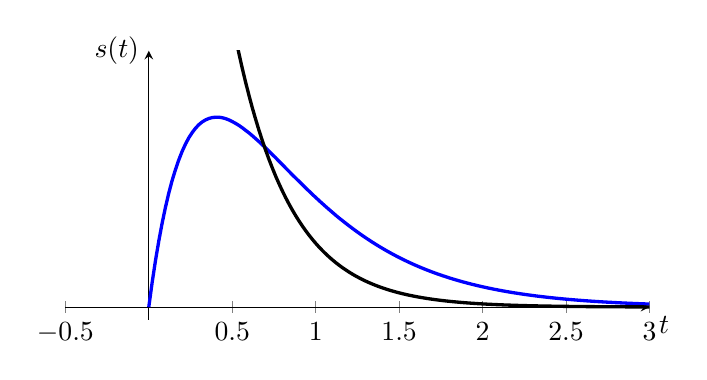
\begin{tikzpicture}
        \begin{axis}[
        scaled y ticks = false,
        height=5cm,
        width=9cm,
        axis x line=center,
        axis y line=center,
        xmin=-0.5,
        xmax=3.0,
        ymin=-0.01,
        ymax=0.2,
        xlabel={$t$},
        ylabel={$s(t)$},
        xlabel style={below right},
        ylabel style={left},
        yticklabels={0,$s(0)=2$},
        ytick={0,2.0},
        y tick label style={anchor=east}
        ]
        \addplot [very thick,color=blue,domain=0:10, samples=501]
        {exp(-2*x)-exp(-3*x)};
        \addplot [very thick,color=black,domain=0:10, samples=501]
        {exp(-3*x)};
        \end{axis}
    \end{tikzpicture}
\end{center}

\newpage
%%%%%%%%%%%%%%%%%%%%%%%%%%%%%%%%%%%%%%%%%%%%%%%%%%%%%%%%%%%%%%%%%%%%%%%%%%%%%%%%
\question{}
%%%%%%%%%%%%%%%%%%%%%%%%%%%%%%%%%%%%%%%%%%%%%%%%%%%%%%%%%%%%%%%%%%%%%%%%%%%%%%%%
\textbf{(3) $\devi{s(t)}{2} + 2\devi{s(t)}{} + s(t)=e(t)$ 
avec $\devi{s(0)}{}=s(0)=0$ et $e(t) = e^{-2t}$}
La transformée de Laplace de l'équation différentielle donne :
\begin{align*}
    p^2S(p)+2pS(p)+S(p)&=E(p) \\
    S(p)&=\dfrac{1}{p^2+2p+1}E(p)
\end{align*}
La fonction de transfert est donné par la fraction rationnelle :
$$
H(p)=\dfrac{1}{p^2+2p+1}
$$
le pôle de $H(p)$ est $p_1=-1$ qui est une racine double
$$
S(p) = \dfrac{1}{(p+1)^2}E(p)
$$
pour $e(t)=e^{-2t}$, $E(p)=\dfrac{1}{p+2}$
$$
S(p)=\dfrac{1}{(p+1)^2(p+2)}
$$
décomposons $S(p)$ en élément simple:
$$
S(p)=\dfrac{A}{p+1}+\dfrac{B}{(p+1)^2}+\dfrac{C}{(p+2)}
$$
$$
A(p^2+3p+2)+B(p+2)+C(p+1)^2=1
$$
$$
\begin{cases}
     A+C&=0 \\
    3A+B+2C&=0 \\
    2A+2B+C&=1
\end{cases}\Longrightarrow
\begin{cases}
    A=-1\\
    B=1\\
    C=1
\end{cases}
$$
$$
S(p)=-\dfrac{1}{p+1}+\dfrac{1}{(p+1)^2}+\dfrac{1}{(p+2)}
$$
la transformée inverse donne :
$$
s(t) = \laplacei{S(p)}= -e^{-t}+te^{-t}+e^{-2t} = (t-1)e^{-t}+e^{-2t}
$$
\begin{center}
\tikzsetnextfilename{ex_3_3_corrige-chap0-ext}
    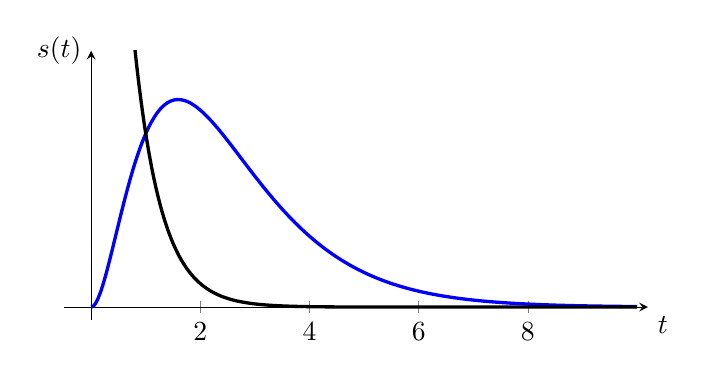
\begin{tikzpicture}
        \begin{axis}[
        scaled y ticks = false,
        height=5cm,
        width=9cm,
        axis x line=middle,
        axis y line=middle,
        xmin=-0.5,
        xmax=10.2,
        ymin=-0.01,
        ymax=0.2,
        xlabel={$t$},
        ylabel={$s(t)$},
        xlabel style={below right},
        ylabel style={left},
        yticklabels={0,$s(0)=2$},
        ytick={0,2},
        xtick={0,2,4,6,8},
        xticklabels={0,2,4,6,8},
        y tick label style={anchor=east}
        ]
        \addplot[very thick,color=blue,domain=0:10 , samples=501]
        {(x-1)*exp(-x)+exp(-2*x)};
        \addplot[very thick,color=black,domain=0:10, samples=501]
        {exp(-2*x)};
        \end{axis}
    \end{tikzpicture}
\end{center}

\newpage
%%%%%%%%%%%%%%%%%%%%%%%%%%%%%%%%%%%%%%%%%%%%%%%%%%%%%%%%%%%%%%%%%%%%%%%%%%%%%%%%
\question{}
%%%%%%%%%%%%%%%%%%%%%%%%%%%%%%%%%%%%%%%%%%%%%%%%%%%%%%%%%%%%%%%%%%%%%%%%%%%%%%%%
\textbf{(4) $\devi{s(t)}{2} + \devi{s(t)}{} + s(t) = e(t)$ 
avec $\devi{s(0)}{}=s(0)=0$ et $e(t) = 1$}}
La transformée de Laplace de l'équation différentielle donne :
\begin{align*}
    p^2S(p)+pS(p)+S(p)&=E(p) \\
    S(p)&=\dfrac{1}{p^2+p+1}E(p)
\end{align*}
La fonction de transfert est donné par la fraction rationnelle :
$$
H(p)=\dfrac{1}{p^2+p+1}
$$
les pôles de $H(p)$ sont deux complexes conjugués: 
$p_{1,2}=-\dfrac{1}{2}\pm j\dfrac{\sqrt{3}}{2}$
$$
S(p) = \dfrac{1}{\left(\left(p+\dfrac{1}{2}\right)^2+
       \dfrac{3}{4}\right)}E(p)
$$
pour $e(t)=1$, $E(p)=\dfrac{1}{p}$
$$
S(p) =\dfrac{1}{p\left(p^2+p+1\right)}
$$
décomposons $S(p)$ en élément simple:
$$
S(p)=\dfrac{A}{p}+\dfrac{Bp+C}{\left(p^2+p+1\right)}
$$
$$
A=\lim\limits_{p \rightarrow 0} pS(p) = 1
$$
\begin{align*}
    p^2+p+1 + Bp^2+Cp &= 1 \\
    \begin{cases}
        B&=-1\\
        C&=-1
    \end{cases}
\end{align*}
\begin{align*}
    S(p)&=\dfrac{1}{p}-\dfrac{p-1}{\left(p^2+p+1\right)} \\
    S(p)&=\dfrac{1}{p}-\dfrac{p}{\left(\left(p+\dfrac{1}{2}\right)^2+
          \dfrac{3}{4}\right)}-
          \dfrac{1}{\left(\left(p+\dfrac{1}{2}\right)^2+\dfrac{3}{4}\right)}\\
    S(p)&=\dfrac{1}{p}-\dfrac{p+\dfrac{1}{2}}
                       {\left(\left(p+\dfrac{1}{2}\right)^2+
                                      \dfrac{3}{4}\right)}-
                       \dfrac{\dfrac{1}{2}}{\left(\left(p+\dfrac{1}{2}\right)^2+
                              \dfrac{3}{4}\right)}\\
    S(p)&=\dfrac{1}{p}-\dfrac{p+\dfrac{1}{2}}
                             {\left(\left(p+\dfrac{1}{2}\right)^2+
                                            \dfrac{3}{4}\right)}-
                       \dfrac{1}{\sqrt{3}}\dfrac{\dfrac{\sqrt{3}}{2}}
                       {\left(\left(p+\dfrac{1}{2}\right)^2+
                                      \dfrac{3}{4}\right)}
\end{align*}
la transformée inverse donne :
$$
s(t) = \laplacei{S(p)}=
1-e^{-\frac{t}{2}}\cos{\left(\dfrac{\sqrt{3}}{2}t\right)}-
\dfrac{1}{\sqrt{3}}e^{-\frac{t}{2}}\sin{\left(\dfrac{\sqrt{3}}{2}t\right)}
$$

\begin{center}
\tikzsetnextfilename{ex_3_4_corrige-chap0-ext}
    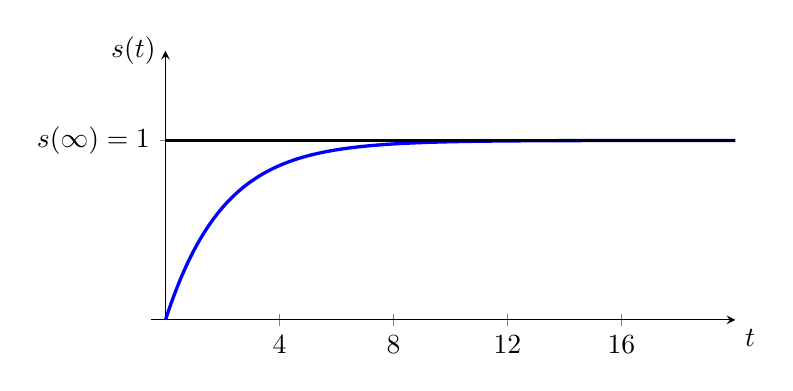
\begin{tikzpicture}
        \begin{axis}[
        scaled y ticks = false,
        height=5cm,
        width=9cm,
        axis x line=center,
        axis y line=center,
        xmin=-0.5,
        xmax=20.0,
        ymin=0.0,
        ymax=1.5,
        xlabel={$t$},
        ylabel={$s(t)$},
        xlabel style={below right},
        ylabel style={left},
        yticklabels={0,$s(\infty)=1$},
        xticklabels={0,4,8,12,16},
        ytick={0,1.0},
        xtick={0,4,8,12,16},
        y tick label style={anchor=east}
        ]
        \addplot [very thick,color=blue,domain=0:20, samples=201]
        {1-exp(-x/2)*cos(sqrt(3)/2*x)-(1/sqrt(3))*exp(-x/2)*sin(sqrt(3)/2*x)};
        \addplot [very thick,color=black,domain=0:20, samples=11]{1};
        \end{axis}
    \end{tikzpicture}
\end{center}

\newpage 
%%%%%%%%%%%%%%%%%%%%%%%%%%%%%%%%%%%%%%%%%%%%%%%%%%%%%%%%%%%%%%%%%%%%%%%%%%%%%%%%
%%%%%%%%%%%%%%%%%%%%%%%%%%%%%%%%%%%%%%%%%%%%%%%%%%%%%%%%%%%%%%%%%%%%%%%%%%%%%%%%
\exercice{Transformée de Laplace d'une fonction périodique}
%%%%%%%%%%%%%%%%%%%%%%%%%%%%%%%%%%%%%%%%%%%%%%%%%%%%%%%%%%%%%%%%%%%%%%%%%%%%%%%%
%%%%%%%%%%%%%%%%%%%%%%%%%%%%%%%%%%%%%%%%%%%%%%%%%%%%%%%%%%%%%%%%%%%%%%%%%%%%%%%%

%%%%%%%%%%%%%%%%%%%%%%%%%%%%%%%%%%%%%%%%%%%%%%%%%%%%%%%%%%%%%%%%%%%%%%%%%%%%%%%%
\question{}
%%%%%%%%%%%%%%%%%%%%%%%%%%%%%%%%%%%%%%%%%%%%%%%%%%%%%%%%%%%%%%%%%%%%%%%%%%%%%%%%
%Déterminer $f_0(t)$ en fonction de $g_0(t)$. 
%Donner la transformée de Laplace de $f_0(t)$.
\tikzsetnextfilename{ex_4_1_corrige-chap0-ext}
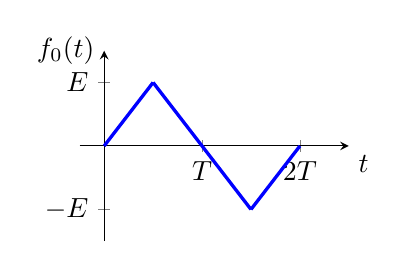
\begin{tikzpicture}
        \begin{axis}[
        height=4cm,
        width=5cm,  
        axis x line=center,
        axis y line=center,
        xmin=-2,
        xmax=20,
        ymin=-1.5,
        ymax=1.5,
        xlabel={$t$},
        ylabel={$f_0(t)$},
        xlabel style={below right},
        ylabel style={left},
        yticklabels={$-E$,$E$},
        ytick={-1,1},
        y tick label style={anchor=east},
        xticklabels={$T$,$2T$},
        xtick={8,16},
        x tick label style={below}
        ]
        \addplot[very thick,color=blue,domain=0:4, samples=101]{0.25*x};
        \addplot[very thick,color=blue,domain=4:12, samples=101]{-0.25*x+2};
        \addplot[very thick,color=blue,domain=12:16, samples=101]{0.25*x-4};
        \end{axis}
\end{tikzpicture}
\tikzsetnextfilename{ex_4_2_corrige-chap0-ext}
\begin{tikzpicture}
        \begin{axis}[
        height=4cm,
        width=5cm,  
        axis x line=center,
        axis y line=center,
        xmin=-2,
        xmax=20,
        ymin=-1.5,
        ymax=1.5,
        xlabel={$t$},
        ylabel={$f_0(t)$},
        xlabel style={below right},
        ylabel style={left},
        yticklabels={$-E$,$E$},
        ytick={-1,1},
        y tick label style={anchor=east},
        xticklabels={$T$,$2T$},
        xtick={8,16},
        x tick label style={below}
        ]
        \addplot [very thick,color=col4,domain=-2:0, samples=101]{0.01};
        \addplot [very thick,color=col4,domain=0:4, samples=101]{0.25*x};
        \addplot [very thick,color=col4,domain=4:8, samples=101]{-0.25*x+2};
        \addplot [very thick,color=col4,domain=8:20, samples=101]{0.01};
        \addplot [very thick,color=col3,domain=-2:8, samples=101]{-0.01};
        \addplot [very thick,color=col3,domain=8:12, samples=101]{-0.25*x+2};
        \addplot [very thick,color=col3,domain=12:16, samples=101]{0.25*x-4};
        \addplot [very thick,color=col3,domain=16:20, samples=101]{-0.01};
        \end{axis}
\end{tikzpicture}
$$
\color{blue}f_0(t)=\color{col4}g_0(t)\color{col3}-g_0(t-T)
$$
où $g_0(t)$ est la fonction \og dent de scie\fg construite précédemment.
$$
F_0(p)=\laplace{f_0(t)}=G_0(p)(1-e^{-Tp})
=\dfrac{2E}{T}\dfrac{(1-e^{-Tp/2})^2}{p^2}(1-e^{-Tp})
$$
\begin{align*}
    F(p)&=\dfrac{F_0(p)}{1-e^{-2Tp}} \\
    F(p)&=\dfrac{2E}{Tp^2}\dfrac{(1-e^{-Tp/2})^2(1-e^{-Tp})}{1-e^{-2Tp}}\\
    F(p)&=\dfrac{2E}{Tp^2}\dfrac{(1-e^{-Tp/2})^2(1-e^{-Tp})}{1-e^{-2Tp}}
                          \dfrac{(1+e^{-Tp})}{(1+e^{-Tp})}\\
    F(p)&=\dfrac{2E}{Tp^2}\dfrac{(1-e^{-Tp/2})^2}{(1+e^{-Tp})}\\
    F(p)&=\dfrac{2E}{Tp^2}\dfrac{(1-2e^{-Tp/2}+e^{-Tp})}{(1+e^{-Tp})}\\
    F(p)&=\dfrac{2E}{Tp^2}\left(1-\dfrac{2e^{-Tp/2}}{(1+e^{-Tp})}\right)
         =\dfrac{2E}{Tp^2}\left(1-\dfrac{e^{-Tp/2}}{e^{-Tp/2}}
                                  \dfrac{2}{(e^{Tp/2}+e^{-Tp/2})}\right)\\
\Aboxed{F(p)&=\dfrac{2E}{Tp^2}\left(1-\dfrac{1}{\cosh{\frac{Tp}{2}}}\right)}
\end{align*}
%%%%%%%%%%%%%%%%%%%%%%%%%%%%%%%%%%%%%%%%%%%%%%%%%%%%%%%%%%%%%%%%%%%%%%%%%%%%%%%%
\exercice{Cartes des pôles et zéros}
%%%%%%%%%%%%%%%%%%%%%%%%%%%%%%%%%%%%%%%%%%%%%%%%%%%%%%%%%%%%%%%%%%%%%%%%%%%%%%%%


%%%%%%%%%%%%%%%%%%%%%%%%%%%%%%%%%%%%%%%%%%%%%%%%%%%%%%%%%%%%%%%%%%%%%%%%%%%%%%%%
%%%%%%%%%%%%%%%%%%%%%%%%%%%%%%%%%%%%%%%%%%%%%%%%%%%%%%%%%%%%%%%%%%%%%%%%%%%%%%%%
%%%%%%%%%%%%%%%%%%%%%%%%%%%%%%%%%%%%%%%%%%%%%%%%%%%%%%%%%%%%%%%%%%%%%%%%%%%%%%%%
%%%%%%%%%%%%%%%%%%%%%%%%%%%%%%%%%%%%%%%%%%%%%%%%%%%%%%%%%%%%%%%%%%%%%%%%%%%%%%%%
%exercice_chap0_corrige.tex

%\normalsize
